\documentclass[letterpaper,12pt]{report}
\usepackage[english]{babel}							%For internationalization
\usepackage[utf8]{inputenc}							%For character encoding
\usepackage{amsmath}								%For mathematical typesetting
\usepackage{amssymb}								%For mathematical typesetting
\usepackage{graphicx}								%For handling graphics
\usepackage[top=1in, bottom=1in, left=1.5in, right=1in]{geometry}	%Sets required thesis margins
\usepackage[nodisplayskipstretch,doublespacing]{setspace} 		%Sets required thesis double spacing
\usepackage{titlesec} 								%Used to easily redefine section title styles
\usepackage{listings}								%Code formatting
\usepackage[nottoc,numbib]{tocbibind}						%Used to include bib in toc and correct the page number

\newcommand{\be}{\begin{equation}}
\newcommand{\ben}[1]{\begin{equation}\label{#1}}
\newcommand{\ee}{\end{equation}}
\newcommand{\aomega}{\overset{\sim}{\omega}}				%Approximate omega

\title{Vortex Dominated Flows: A High-Order, Conservative Eulerian Simulation Method}
\author{Josh Bevan}
\date{\today}

%Set section formats so chapters, sections, and subsections are 14ish pt
\titleformat{\section}{\large\bfseries}{\thesection}{1em}{}
\titleformat{\subsection}{\normalsize\bfseries}{\thesubsection}{1em}{}
\titleformat{\chapter}{\large\bfseries}{\thechapter}{1em}{}
	\titlespacing*{\chapter}{0pt}{.7in}{0pt} 				%Add whitespace above chapter title to get a 2in margin

\renewcommand{\floatpagefraction}{.8}					%Allow more text on pages with floats

%Frontmatter----------------------------------------------------------------------
\begin{document}
\begin{center}
\pagenumbering{roman} %Roman numbering for frontmatter
\setcounter{page}{2}
\large VORTEX DOMINATED FLOWS: A HIGH-ORDER, CONSERVATIVE EULERIAN SIMULATION METHOD\\
\vspace{1cm}\normalsize BY\\
\vspace{1cm}\normalsize JOSHUA BEVAN

\vspace{1cm} \normalsize ABSTRACT OF A THESIS SUBMITTED TO THE FACULTY OF THE\\
DEPARTMENT OF MECHANICAL ENGINEERING\\
IN PARTIAL FULFILLMENT OF THE REQUIREMENTS\\
FOR THE DEGREE OF\\
MASTER OF SCIENCE\\
UNIVERSITY OF MASSACHUSETTS LOWELL\\
2015\\
\end{center}
Thesis Supervisor: David J. Willis\\
Assistant Professor, Department of Mechanical Engineering

\begin{abstract}
\setcounter{page}{3}
%Manual page numbering because 'abstract' is annoying
\thispagestyle{plain} %Needed to show page number as pagestyle was reset to 'empty' when \maketitle is called internally
A high-order, conservative Eulerian method is presented for the simulation of vortex dominated inviscid fluid flows. The primitive variable incompressible Euler equations are recast in the velocity-vorticity form to explicitly enforce conservation of vorticity. The advection of the vorticity is then calculated via a two-step process: the velocity field is first determined by evaluation of the Biot-Savart integral, and then a line-based discontinuous Galerkin (DG) Eulerian spatial discretization scheme is applied to accurately advect the vorticity field. The accuracy and convergence of this method is examined for test cases where an analytical solution exists, as well as more challenging test cases which lack an analytical solution. The influence the velocity field discretization has on the performance of the method is of particular interest.

It is shown that the order of accuracy of the velocity field must be at least the same order as the vorticity field to maintain desired convergence. The error in the calculated velocity field is heavily influenced by the approximation taken in estimating the Biot-Savart integral. In particular, the approximation of the desingulariztion of the Biot-Savart integral to deal with singularities in the self-influence of an element leads to a careful balance. The error in the calculated velocity introduced by the desingularization must be balanced with the ameliorative effect the desingularization has on the convergence of the numerical quadrature applied to the Biot-Savart integral. Proper choice of parameters leads to nearly optimal convergence of the overall method in the analytical test, and high-order convergence in the qualitative test case.
\end{abstract}

 \setcounter{page}{4}%Manual page numbering because 'abstract' is annoying
\chapter*{Acknowledgments}
Foremost, I would like to express my sincere gratitude to my advisor Prof. David Willis without whom this thesis, and indeed my graduate career would not exist. His enthusiasm and approachable style spurred me into pursuing computational science, when a semester before in my undergraduate degree I could not have imagined the path I would eventually take. His patience, wisdom, advice, and knowledge were instrumental in shaping both this thesis, as well as myself as a student.

I would also like to thank the other members of my committee Prof. Juan Pablo Trelles and Prof. Per-Olof Persson. Their combined knowledge, insight, and feedback were a huge asset. Their questions and comments sharpened the quality of the thesis as well as my own thinking on the subject. In particular, Prof. Persson's work on Line-DG was notably useful in the easy extension to multiple dimensions of the solver. I would also like to thank Prof. Trelles for his tutelage during my graduate studies and his introduction to me of the software package PETSc, which gave me a great appreciation for clear and concise thought in the execution of a software code.

Finally, I would also like to say a belated thank you to my undergraduate advisor Prof. Peter Avitabile who was instrumental in my success as an undergraduate student. His patience, guidance, and understanding were instrumental to my success as a student and his practical and knowledgeable skill as an instructor enriched my own knowledge.

\begin{singlespace} %Tables should be single spaced
\tableofcontents
\listoftables
\addcontentsline{toc}{section}{List of Tables}
\listoffigures
\addcontentsline{toc}{section}{List of Figures}
\end{singlespace}

%Here we change the pagestyle so that the page number appears top right. We need to redefine the \chapter command to change the default pagestyle from 'plain' to 'myheadings'
\pagestyle{myheadings}
\makeatletter
\renewcommand\chapter{\if@openright\cleardoublepage\else\clearpage\fi
                    \thispagestyle{myheadings}% original style: plain
                    \global\@topnum\z@
                    \@afterindentfalse
                    \secdef\@chapter\@schapter}
\makeatother

%Mainmatter-----------------------------------------------------------------------
\chapter{Introduction}
\pagenumbering{arabic} %Reset to arabic numbering for mainmatter
\section{Velocity-Vorticity equation}
Direct solution of Navier-Stokes is impractical for many fluid problems and where possible simplifications should be made; one such possibility is for vortex dominated flows. It is possible to recast Navier-Stokes from a primitive variable form ($u,v,p$) to a velocity-vorticity ($u,v,\omega$) form. This has several advantages: explicit conservation of vorticity, elimination of pressure terms (for incompressible flows), and reduction of required simulated degrees of freedom to just those that form the vorticity support. However, the additional complications are added to the technique when local boundary conditions must be imposed (e.g. solid bodies in the domain). For inviscid and incompressible flows the vorticity transport equation is:
\ben{VV3D} \frac{\partial \omega}{\partial t} + u \cdot \nabla \omega - \omega \cdot \nabla u = S(x,t)\ee

Traditionally vorticity and vortex based simulation techniques take advantage of Helmholtz and Kelvin's theorems; vorticity exists as material surfaces, lines, etc. and therefore a Lagrangian approach is natural. Typically the vorticity is discretized into vortex particles, lines, or sheets at which point advection becomes trivial, one merely needs to calculate the velocity field at each particle and step forward in time \cite{Strain1996,MoussaCarley2008,KoumLeonard1995}. Several monographs exist that decribe the details and advantages of Lagrangian vortex methods \cite{Lugt1983,Saffman1992,Speziale1987}.

\section{Lagrangian Methods}
There are several variations of Lagrangian methods depending on how the vorticity is discretized; point vortex methods were the earliest with the work of Rosenhead \cite{Point1} in 2D with singular point vortices, which was later built upon and improved \cite{Point2,Point3,Point4,Point5,Point6}. Higher dimensional discretizations take the form of vortex line \cite{Line1,Line2,Line3,Line4}, sheets \cite{Sheet1,Sheet2,Sheet3}, and volumes \cite{Volumes1,Volumes2,Volumes3}.

The velocity field due to the vorticity is usually calculated from solving the Poisson problem \cite{MiscMeth1}, or through inversion of the Poisson problem via evaluation of the Biot-Savart integral \cite{Saffman1992}. There are several challenges with evaluation of the velocity: boundary conditions in the Poisson solution method, and singularities in the Biot-Savart volume integral method. Typically Lagrangian point vortex codes must de-singularize the kernel \cite{Rosenhead1930,Moore1972}. Direct summation for the velocity field has a $\mathcal{O}(N^2)$ complexity. Tree-codes \cite{LindsayKrasny2001} and Fast Multipole Methods (FMM) \cite{Strain1997} are common ways of achieving a more efficient calculation.

The convergence of vortex methods was proven early on for 2D \cite{Convg2D} and was later extended to 3D \cite{Convg3D}.

\section{Lagrangian Method Difficulties}
Lagrangian point methods present several problems. Point disorganization can occur as the fluid evolves, this typically requires temporary meshing to recondition the discretization. This has been handled with various methods; recalculation of the quadrature weights at each time step \cite{Remesh2,Remesh3}, regridding/rezoning \cite{Remesh4}, and remeshing \cite{Remesh5} among them. Additionally, most Lagrangian approaches are limited to low order; careful point locations must be chosen and maintained through frequent remeshing etc. in order to achieve high-order convergence \cite{Strain1997}.

\section{Existing Eulerian codes}
In comparison, Eulerian approaches to vortex methods tend to be less common. Work has been done for viscous flows with solid bodies; both stationary \cite{MiscMeth3} and moving \cite{MiscMeth2}. Both of these solve the streamfunction-vorticity formulation, not the velocity-vorticity formulation. The velocity-vorticity formulation has been solved by an Eulerian approach by others \cite{MiscMeth4}.A notable example of an Eulerian approach to the velocity-vorticity formulation is the work of Brown et al. \cite{Brown2000} who adapted the velocity-vorticity approach to a low order Finite Volume (FV) solver. Later they were able to extend their method to be accelerated via a FMM \cite{Brown2004}. However, like most FV approaches, to extend to high order solution approximations requires extended stencils that ultimately limit the geometrical freedom of the mesh. Steinhoff et al. also used an Eulerian approach, but solved a modified form of the inviscid Euler equations with ``vorticity confinement'' rather than the velocity-vorticity equation \cite{SteinhoffUnderhill1994}.
%
\section{Proposed Method}
\subsection{Alternate Advective Methods}
The desire to resolve fine vortical structures motivates the need for a high order solver. Considering the challenges associated with achieving a high order Lagrangian method and the preliminary success of Brown et al.'s low order method, it is natural to attempt a high order Eulerian vorticity-velocity method, but what of the spatial discretization choice?

Finite difference methods suffer from similar problems as FV with extended stencils, as well as not being explicitly conservative. A finite element approach is ill-suited to the hyperbolic nature of vorticity advection. Spectral methods are promising, but for sparse vorticity domains are less-efficient due to the global support of the harmonic bases. However, discontinuous Galerkin (DG) methods \cite{HestWar} are a natural choice; they are conservative, able to take advantage of vorticity sparseness, are well-suited to handle advection via intelligent choice of a numerical flux function, and have bases with local/compact support.

For domains free of impinging bodies a hexahedral mesh with a tensor product grid of interpolation points is convenient to implement. This permits the use of a line-DG \cite{Persson2013} approach that considerably simplifies multi-dimensional cases by allowing reuse of 1D methods. A 2D domain will be considered to evaluate whether the method is practical, as well as to limit solution times to those that are reasonable on a workstation. This has the advantage of removing the vortex stretching term and reducing the vorticity to a scalar. The resultant partial differential equation (PDE) takes on the familiar form of a scalar conservation law.

\subsection{Velocity Field Fidelity}
Unlike Lagrangian methods where advection is trivial, or Brown's method \cite{Brown2004} which is at low order, the necessary fidelity of the velocity field to maintain a particular global convergence rate that one would expect from the order of the vorticity field is not immediately obvious. The method by which one recovers the velocity field is decoupled from the advective solver, which has no a priori knowledge or assumptions about the quality of the velocity field approximation. 

To maintain maximum flexibility for investigative purposes and to remove as much approximation error as possible the velocity field for validation of the underlying method is calculated via direct evaluation of the Biot-Savart integral.

\section{Thesis Goals and Structure}
The overarching thesis goal is the development of a high-order solver capable of modeling inviscid incompressible vorticity-dominated flows in 2D. For simplicity only unconstrained flow free of solid bodies within the domain is considered in the present solver. In order to accomplish this several ancillary goals must be achieved: construction of a high-order advective solver capable of mixed order flux handling, and a high-order Biot-Savart evaluation routine that is as efficient as can be achieved within the bounds of a direct summation approach.

At it's conclusion the chief contributions will be: a complete high-order method for velocity-vorticity inviscid flow that integrates all necessary subsystems, validation of the solver and the underlying Eulerian vortex approach; and evaluation of the convergence, error, and performance of the method and solver.

In Chapter 2, a brief overview of the underlying theory of the velocity-vorticity formulation, velocity evaluation, the Biot-Savart  kernel and the discontinuous Galerkin method are covered. The extension of one-dimensional DG methods to 2D via a line-DG \cite{Persson2013} style method will also be reviewed. 

In Chapter 3 the methodology taken to construct a high-order Eulerian velocity-vorticity is covered. Chief among the concerns are the spatial basis, choice of interpolation, and numerical integration of the interpolation.

Chapter 4 covers solver specific implementation details. An introductory overview of the solver structure is first laid out. Then, formation of the semi-discrete system, along with the development of some specialized tools are addressed. A high-order velocity evaluation method is laid out, as well as some computation-saving modifications. Explicit time-stepping via a Runge-Kutta method optimized for the spectra of the DG operator is briefly reviewed.

In Chapter 5 a test plan is laid out for validation and investigation of the overall solver and method. Results of the validation tests, convergence studies, and diagnostics are presented.

In Chapter 6 discusses the successful validation of the method, as well as the high-order convergence rates achieved. The dependency of a successful solution upon flow conditions and generation of small non-physical artifacts are also discussed.

Chapter 7 concludes the thesis as well as suggests several next steps that should be taken to improve the generality and performance of the method.

Appendix A presents the specific implementation details necessary to implement the solver practically and efficiently. Several Matlab functions and routines are presented that either makeup the solver itself, or necessary auxiliary tools that are tangentially needed.

%------------------------------------
\chapter{Theory}
\section{Navier-Stokes: Velocity-vorticity form}
The Navier-Stokes momentum equation is
 \be \rho \left(\frac{\partial \mathbf{u}}{\partial t} + \mathbf{u} \cdot \nabla \mathbf{u} \right) = -\nabla p + \mu \nabla^2 \mathbf u + \tfrac13 \, \mu \nabla (\nabla\cdot\mathbf{u}) \ee
where $u$ is the velocity field, $p$ is the pressure, and $\rho$ is the density. If we restrict ourselves to incompressible flows and define the quantity \textit{vorticity} as
\be \mathbf{\omega} = \nabla \times \mathbf{u} \ee
Then the traditional form of the Navier-Stokes equations can be recast
\ben{VV3D} \frac{\partial \omega}{\partial t} +  \mathbf{u} \cdot \nabla \omega - \omega \cdot \nabla  \mathbf{u} = S(x,t)\ee
where we collect viscous generation of vorticity in $S$.

There are several benefits to the recast $\mathbf{u}$-$\omega$ form:
\begin{enumerate}
\item Explicit conservation of vorticity. The vorticity is recoverable from the primitive variable Navier-Stokes, but the diffusive nature of most upwinded advection means coherent vortical structures are quickly smeared.
\item Frequently the distribution of the vorticity is quite sparse. The primitive variable form requires the velocity and pressure be evaluated over the whole domain. In comparison, the velocity-vorticity form only requires velocity to be evaluated in areas of non-zero vorticity. In areas where there is no vorticity, nothing needs to be advected; hence, no velocity evaluation is required in these areas. The sparser and more concentrated the vorticity, the larger the gap in performance between the two forms; this is especially true in 3D domains where the scaling from surfaces to volumes gives even greater opportunity for empty local regions in the domain. 
\item The primitive-variable form requires the pressure be  solved via a separate elliptic equation. The velocity-vorticity form is absent the pressure and automatically ensures satisfaction of continuity.
\end{enumerate}

For 2-D distributions of vorticity, several simplifications can be made. The originally vectorial vorticity becomes a scalar quantity, all vorticity is directed normal to the plane. As a result, the vortex stretching term in  Eqn.\,\eqref{VV3D} becomes zero. The only non-zero component of $\omega$ is in the z-direction, however the gradient of the velocity field is zero in the z-direction, so the product is therefore zero. The result is
\ben{VV2D} \frac{\partial \omega}{\partial t} + u \cdot \nabla \omega = S(x,t)\ee
or if instead the second term is expressed in terms of the flux of the vorticity (where $f_i(\omega)=u_i\,\omega$):
\ben{VV2DB} \frac{\partial \omega}{\partial t} + \frac{\partial f}{\partial x_i}= S(x,t)\ee

\section{Velocity Field Evaluation: The Biot-Savart Integral}
Since $\omega$ is the quantity of interest in the flowfield solution, the question must be posed: how does one determine the velocity field? For an incompressible 2D or 3D flow we can relate the velocity and vorticity by:
\be \nabla^2 u = -\nabla \times \omega \ee
If inverted, the Biot-Savart integral is obtained
\ben{BS} u(x^*) = \int_\Omega K(x^*,x) \times \omega(x) dx \ee
where $x^*$ is the point we wish to evaluate the velocity, $x$ is the coordinate in regions of non-zero vorticity, and $K(x^*,x)$ is the singular Biot-Savart kernel \cite{BealeMajda}
\ben{BSkern} K(x^*,x) = \frac{-1}{2 \pi} \frac{x^*-x}{|x^*-x|^2} \ee

There are several important points to note that are a consequence of this inversion. First, rather than solving the Poisson equation for the entirety of the domain we choose to evaluate the velocity only at regions where it is needed. For the purposes of advecting the velocity we will only need velocities near the vorticity itself. However, if the number of required velocity evaluation points is roughly proportional to the $N$ degrees of freedom of our vorticity approximation, then it is expected the velocity calculations will scale as $\mathcal{O}(N^2)$.

There are numerous methods to reduce the computational complexity of similar N-body type problems to $\mathcal{O}(NlogN)$ or $\mathcal{O}(N)$. Cyclic reduction \cite{SchumannSweet1976}, tree-codes \cite{LindsayKrasny2001,BarnesHut1986}, and FMM \cite{GreengardRokhlin1987} are all possibilities. However, because the velocity field calculation method is decoupled from the PDE governing vorticity advection, there is no \textit{a priori} assurance that the velocity calculated is of sufficient fidelity to ensure convergence of the overall method. Even if it is sufficient for convergence, there is no guarantee the convergence would be at the order one might expect based on solely the discretization. For maximum flexibility in investigating this dependency of overall convergence on the calculated velocity field we shall eschew more efficient techniques so that we can directly control the fidelity of the velocity field.

\section{Kernel Desingularization} 
The second point to consider regarding the Biot-Savart integral is the singular nature of the exact kernel. Lagrangian point vortex methods have the benefit that the singularity and it's associated non-physical velocities occur in a relatively small region; they assume that the advective effect of the point vortex on itself is negligible. Generally, self-influence merely results in solid body rotation. This is the approach taken by early methods \cite{Point1}. While easy to implement, it results in large, non-physical velocities when two point vortices approach near each other. The other issue with this approach is poor convergence and accuracy of the resulting velocity field off particle paths as described by Beale and Majda \cite{BealeMajda}.

One may attempt to desingularize the Biot-Savart kernel  by introducing a core function $\eta(^z/_{\delta})$. Heuristically, the point vortex is now replaced by a finite size vortex blob described by $\eta(r)$, with characteristic radius $\delta$. Analytically, the point vortex is a delta function; core functions are desingularized approximations that converge to the delta function as $\delta \rightarrow 0$. Traditionally the core function is convolved with the Biot-Savart kernel to yield a desingularized kernel $K_{\delta}$.
\ben{DesingBS} K*\eta(r) = K_{\delta} \ee

The choice of a core function and a characteristic radius has important implications on the accuracy and convergence of a Lagrangian point vortex method. Choosing a cutoff radius too small and there is insufficient smoothing, too large and the vorticity discretization is spatially smeared. The choice of a core function is also nuanced: good approximations of the delta function should preserve both the volume and moments of the delta function \cite{BealeMajda}.

Strictly positive core functions can only preserve the first moment, those preserving more may become negative in small regions. The more moments that are preserved, the higher order the convergence of the underlying method (assuming adequate choice of cutoff radius and sufficiently smooth flow). One may preserve all moments, permitting spectral convergence, with the caveat being the resulting core function does not have compact support \cite{Hald3}. This precludes the use of a tree-code of FMM. There are a wide range of desingularized kernels available, those tested in the solver are presented here.

The classical choice is the Rosenhead-Moore kernel \cite{Rosenhead1930,Moore1972}. Strictly speaking this kernel does not satisfy convergence proofs as it does not conserve any moments. It is technically a 0th order kernel.
\ben{RMkern} K_{RM} = \frac{1}{2 \pi} \frac{x^*-x}{|z|^2+\delta^2} \ee
where we have substituted $z=x^*-x$.

In \cite{WL} Winckelmans and Leonard derived a high-order algebraic kernel that preserves the first moment of the delta function, with second-order formal convergence.
\ben{WLkern} K_{WL}=\frac{1}{2 \pi} \frac{(z)(|z|^2+2\delta^2)}{(|z|^2+\delta^2)^2} \ee

In \cite{BealeMajda} Beale and Majda extend the super-gaussian core function to explicitly generate arbitrary $m^{th}$ order core functions of the type
\ben{SGkern} K_{BM}= \frac{z}{2 \pi |z|^2} (1-Q^{(m)}(^z\!/_{\delta})e^{^{-z^2}\!/_{\delta^2}} )\ee
where $Q^{(m)}(r)$ are Laguerre polynomials of $r^2$ normalized to set the first term to 1.

The final set of kernels used are the spectrally convergent set derived from Bessel functions of the first kind. The simplest appears in \cite{WL} as
\ben{PSkern0}  K_{spectral_0}= \frac{z}{2 \pi |z|^2} (1-J_0(\frac{z}{\delta})) \ee
with a more involved alternative from \cite{HaldReview}
\ben{PSkern2}  K_{spectral_2}= \frac{z}{2 \pi |z|^2} \left[1-\frac{8}{45(z/\delta)^2}(4J_2(\frac{4z}{\delta})-5J_2(\frac{2z}{\delta})+J_2(\frac{z}{\delta}))\right] \ee
these have the advantage that \textit{all} moments are conserved, but they do not have compact support. They are also quite expensive to evaluate due to the Bessel evaluations. For a Lagrangian method this is a serious disadvantage (especially if one wishes to employ a FMM); however for an Eulerian method the vorticity solution points are fixed, so the kernel values need only be calculated once and re-used.

The high-order Eulerian approach taken here means that while the Biot-Savart integral converges, a singularity is always present within any of the extended vorticity patches thanks to self-influence. Conceptually this doesn't present an impossible problem, the integral \textit{does} converge in an analytical sense; practically speaking however a singularity may cause numerical integration procedures to diverge, or at the very least converge quite slowly. The approach taken by Brown \cite{Brown2004} was to use the Rosenhead-Moore kernel, choosing a core size such that the maximum velocity occurred on the face of the finite volume unit. This can be constructed \textit{a priori} because the vorticity is taken as constant across the volume, as is typical in a FV approach. If the vorticity is spatially varying however, the choice of core size is more troublesome. This will be examined in greater detail in the next chapter.

\section{The Discontinuous Galerkin Method}
In order to solve Eqn.\,\eqref{VV2D} we adopt a method-of-lines approach \cite{RKDG}. We will first spatially discretize the system to obtain the semi-discrete system, then we use an explicit time discretization method to march forward in time. Note that Eqn.\,\eqref{VV2D} has the form of a scalar conservation law, with $\omega$ being the conserved quantity. The velocity field that advects the conserved quantity has been calculated by evaluation of the Biot-Savart integral for the current timestep.

Our spatial discretization is at best an approximate solution to Eqn.\,\eqref{VV2D}, that we shall denote as $\aomega(x,t)$. Some residual will remain for the approximate solution of the PDE at any time $t$
\ben{VV2D} \frac{\partial \aomega}{\partial t} + \frac{\partial f}{\partial x_i} = R(x)\ee
where we have shown a 1-D case and omitted vorticity sources for simplicity.

The discontinuous Galerkin (DG) approach was introduced by Reed and Hill to solve the steady-state neutron transport equation in 1973 \cite{ReedHill} and later extended to general linear hyperbolic systems by Lesaint and Raviart \cite{Lesaint}. It attempts to approximately satisfy the PDE in the following way: Seek the best approximation in a finite vector test space $\mathbb{W}_h$  in the $L^2$ norm sense. Minimize the $L^2$ norm by an orthogonal projection of the residual onto $\mathbb{W}_h$. Form a complete basis for $\mathbb{W}_h$ with a set of test functions $\phi_j \in \mathbb{W}_h$, such that the orthogonal projection satisfies:
\be \int_\Omega R(x) \phi_j \;dx = 0 \quad\mbox{for all}\; j\ee
Substituting the residual for our conservation PDE yields:
\be \int_\Omega \frac{\partial \aomega}{\partial t} \, \phi_j \;dx + \int_\Omega \frac{\partial f(\aomega)}{\partial x} \, \phi_j \;dx = 0 \quad\mbox{for all}\; j\ee

Now we go about reconstructing an approximation to the solution by following a common approach \cite{HestWar}. Choose the space of piecewise polynomials for the finite dimensional approximation space, and decompose the global domain into K elements where the local approximation space $\overset{k}{\mathbb{V}}_h$ has basis functions $\overset{k}{\psi}_i(x)$ over the local domain $x \in [x_L, x_R]$ (henceforth we drop the element index $k$ for brevity, except when describing two distinct elements that must be distinguished). Note that continuity of vorticity is not enforced across elements, and that the local approximation spaces for each element are independently defined. Finally, take the Bubnov-Galerkin choice of setting the test space to be the same as the approximation space so that $\phi_j=\psi_i \in \mathbb{V}_h$ if $i=j$. The local Mth order approximation to vorticity takes the form

\be \omega(x,t) \approx \aomega(x,t) = \sum_{i=0}^M a_i(t)\psi_i(x)\ee

where $a_i$ is some set of coefficients that are to be determined. The elemental approximating PDE is then

\be \sum_{i=0}^M \left[ \frac{d a_i(t)}{dt}\int_{x_L}^{x_R}\psi_i(x)  \, \phi_j(x) \;dx \right]
+ \int_{x_L}^{x_R} \frac{\partial f(\aomega)}{\partial x} \, \phi_j \;dx = 0 \ee

To reduce the smoothness requirements on the flux, integrate the second term by parts to yield
\ben{DGtemp} \sum_{i=0}^M \left[ \frac{d a_i(t)}{dt}\int_{x_L}^{x_R}\psi_i(x)  \, \phi_j(x) \;dx \right]
+ f\phi_j(x) \Big|^{x_R}_{x_L} 
- \int_{x_L}^{x_R} f(\aomega) \, \frac{d \phi_j(x)}{d x} \;dx = 0 \ee

The local solution offers no way of recovering the global solution, until one realizes that the flux at the element boundaries is multiply defined between elements. The global solution is allowed to be piecewise discontinuous across boundaries, so there is no guarantee that the flux between neighboring elements would agree. To resolve this (and at the same time recover a global solution) define a numerical flux analogous to a Finite Volume Method that takes as input the vorticity at the adjacent element boundaries. We will use an upwind flux, where defining the average as $\{\!\{\omega^+\}\!\} = \frac{\omega^++\omega^-}{2}$ and the jump as $[[\omega]]=\omega^+-\omega^-$ \cite{HestWar}, yields
\be \hat{f}_{upwind}(x^+,x^-)=u\{\!\{\aomega\}\!\} + \frac{|u|}{2}[[\aomega]]\ee

We would also like to map any element to a computational element by means of a mapping $x=g(X)$ and it's inverse $X=G(x)$. If we set the domain of our computational element to be $X \in [-1, 1]$ and the element size to be $\Delta x = x_R - x_L$, then the mapping is
\be x=g(X)=\frac{X+1}{2}\Delta x + x_L\quad ,\quad X=G(x)=\frac{2(x-x_L)}{\Delta x}+1 \ee

Applying a change of variables using the mapping to Eqn.\,\eqref{DGtemp}, accounting for the numerical flux, and being sure to include the determinant of the Jacobian matrix that results from the mapping ($J=g'(X)=\Delta x/2$) in the first integral:
\ben{DGtemp2} \frac{\Delta x}{2}	\sum_{i=0}^M \left[ \frac{d a_i}{dt}	\int_{-1}^{1}\psi_i  \, \phi_j \;dX \right]
+\hat{f}\phi_j \Big|^{x_R}_{x_L} 
- \int_{-1}^{1} f(\aomega) \, \frac{d \phi_j}{dX} \;dX = 0 \ee
(Note: no determinant of the Jacobian matrix appears in the second integral because one of the basis functions has been differentiated. When the chain rule is applied during the change of variables an extra $1/g'(X)$ appears that cancels out with the $g'(X)$ that occurred from the change of variables on the integral).

We have purposely left the flux in the second integral unevaluated in terms of the basis functions, as well as the choice of basis functions left as undecided. We defer these choices to a more in depth investigation in \S \ref{DGchoice}. We also have developed the equations past the initial PDE in a 1-D form. We will shortly show that the basis coefficients are chosen to be nodal values. The 2-D solution will be recovered following the Line-DG methodology \cite{Persson2013} where each element will be composed of a tensor product of two 1-D discretizations.

%------------------------------------
\chapter{Methodology}
Solver specific implementation details are deferred until the next chapter while we develop method specific choices and numerical machinery. However it is instructive to briefly outline the programmatic flow of the solver.
\section{Preliminary Solver Overview}\label{Pseudo1}
\vspace{-1cm}
\singlespacing
\begin{lstlisting}[language=Matlab]
Define problem parameters
Define solver parameters
Calculate derived solver parameters
Setup intitial conditions
Initialize solver
%Time stepping
for t=0 to end
   if datalog?=yes
      save system state to file and plot
   end
   %Loop through RK stages
   for s=1 to last_stage
      %For elements above threshold
      for each vorticity source
         calculate velocity contributions
      end
      %Calculate semi-discrete system terms
      interpolate element_boundary_vorticity
      calculate numerical_fluxes
      calculate total_surface_flux
      calculate internal_stiffness_flux
		
      vorticity_rate_of_change=...
         internal_stiffness_flux - total_surface_flux
		
      RK_stage= (RK_coeff_a*RK_stage) +...
         (time_step * vorticity_rate_of_change)
      vorticity= vorticity + RK_coeff_b * RK_stage
   end
end
\end{lstlisting}
\doublespacing

%
\section{Method Specific DG Choices} \label{DGchoice}
We now seek to take the general form of Eqn.\,\eqref{DGtemp2} and customize it to suit our needs. There are several choices to be made, the space of the basis, the physical meaning of the basis coefficients, and how the basis is constructed for a 2D domain. We shall take the common choice of the space of polynomials for our basis. Additionally we shall choose our basis coefficients to be local nodal values that our basis interpolates.

One could be tempted to choose a modal basis, but for simplicity of extension a nodal basis allows one to readily expand 1D basis functions to 2D by means of a tensor product of two 1D bases. If the two 1D basis are linearly independent, then the tensor product spans $\mathbb{R}^2$. Furthermore, if the bases are orthogonal to each other then each can be treated separately. To illustrate this we must choose our basis functions; a readily specified choice for interpolation is the Lagrange basis:
\be \psi_i(x) =\ell_i(x) = \prod_{\substack{p=0\\ p\neq i}}^M \frac{x-x_p}{x_i-x_p}\ee
where, M is the order of the basis and the set of points ${x_p}$ are the $M+1$ interpolation points. The interpolatory property of the Lagrange basis means that $\ell_i(x_j) = \delta_{ij}$, so that the value of the function at the interpolation points forms the expansion coefficients:
\be f(x) \approx \sum_{i=0}^M z_i \ell_i(x) \ee

%
\section{Interpolation Node Choice}\label{INC}
It is well known that for moderate orders equispaced interpolation nodes are a poor choice that will suffer from Runge's Phenomenon. To avoid this, nodes that are the roots of an orthogonal polynomial family are commonly adopted; Chebyshev, Legendre, and Legendre-Lobatto are all common choices \cite{Roni}. 

At first one may be tempted to choose the Lobatto points as they include nodes on the extremes of the domain, which are needed for the boundary flux evaluation. There is a minor problem with this however. We would ideally like to collocate our quadrature nodes with our interpolation points, so that they can be reused for any numerical integration. However a Gauss-Lobatto quadrature rule is $2N-1$ order accurate \cite{Roni}. This means if we have the product of two $N$th order polynomials that share the same nodes, a collocated Lobatto quadrature rule is not exact. While this is permissible, there is another point to consider. If the interpolation points are the roots of a single orthogonal polynomial, then the associated Lagrange bases of differing order are orthogonal.

Consider the inner product of two Lagrange polynomials that share the same interpolation nodes which are the roots of the Legendre polynomials, one may rearrange terms to obtain

\be \begin{split} &\int \ell_i(x) \ell_j(x) dx = \int \frac{1}{c_1} \prod_{p\neq i}^M (x-x_p) \frac{1}{c_2}\prod_{q \neq j}^M (x-x_q) \;dx \\ 
&=\frac{1}{c_3} \int  \Big[(x-x_0)...(x-x_{i-1})(x-x_{i+1})...(x-x_M)\Big]\prod_{p \neq j} (x-x_p) \;dx\\
&=\frac{1}{c_3} \int  \Big[(x-x_0)...(x-x_{i-1}) \boldsymbol{(x-x_i)}(x-x_{i+1})...(x-x_M)\Big] \frac{1}{\boldsymbol{(x-x_i)}}\prod_{p \neq j} (x-x_p) \;dx\\
&=\frac{1}{c_3} \int  P_M(x) \pi_{M-2}(x) \;dx= 0\end{split}\ee
where $P_M$ is the Mth order Legendre polynomial and $\pi(x)$ is a $M-2$th order arbitrary polynomial.

The Legendre polynomial is a result of the complete polynomial being reconstructed from it's roots one by one. Since the Legendre polynomials form a complete basis, $\pi(x)$ can be expressed in terms of a sum of them. All of the Legendre terms that appear in this sum are lower order than $P_M$ (and therefore orthogonal to $P_M$), so the integral is zero. For the inner product of the same Lagrange basis for a point $i$, one simply recovers the associated quadrature weight $w_i$ so that in general
\be \int \ell_i(x) \ell_j(x) dx = \delta_{ij} w_j \ee

%
\section{Line-Discontinuous Galerkin}
An important consequence of the tensor basis means that the two basis directions are not coupled except at the interpolation nodes at the intersection of each direction's basis. This is the central idea in the line-DG \cite{Persson2013} approach, a 2D problem is transformed into two 1D problems of the form of Eqn.\,\eqref{DGtemp2}. The 2D time evolution of the overall system is the linear combination of the 1D evolutions; notably the instantaneous rate of change of a particular node is the sum of the rates from each direction. Heuristically, a node can be thought of as a differential element with each direction's basis acting on the respective ``face'' of the node.

We can now use the developed 1D basis in a tensor product to form our 2D basis
\be f(x,y) \approx \left[\sum_{j=0}^L z_j \ell_j(y) \right] \times \left[ \sum_{i=0}^M z_i \ell_i(x) \right] = \sum_{j=0}^M \sum_{i=0}^M z_{ij} \ell_j \ell_i =  \sum_{j=0}^M z_{ij} \ell_j \sum_{i=0}^M  \ell_i \ee
In general the tensor basis could have unequal order along each direction, but for simplicity we use an equal order.

We now substitute our basis into Eqn.\,\eqref{DGtemp2} to get a particular direction's PDE
\ben{DGJoshTemp} \frac{\Delta x}{2}	\sum_{i=0}^M \left[ \frac{d z_{ij}}{dt}	\int_{-1}^{1}\ell_i  \, \ell_j \;dX \right]
+\hat{f}\ell_j \Big|^{x_R}_{x_L} 
- \int_{-1}^{1} f(\aomega) \, \ell_j' \;dX = 0 \ee
We solve the PDE ``line-wise''; we form the tensor product of the chosen 1D interpolation nodes, as shown in \ref{fig:DGtensorSplit}. In this example we would solve 10 $\times$ 1D problems: 5 along the $x$-direction and 5 along $y$-direction. The solution of Eqn.\,\eqref{DGJoshTemp} for any one of these 1D problems yields the rate of change of vorticity for all nodes along that line. This only accounts for advection along one-direction; the complimentary perpendicular line intersecting at a node on the first line also contributes. In example figure \ref{fig:DGtensorSplit} the rate of change of the vorticity at the node at the intersection of the two lines is the sum of rates of changes from each line. In general the rate of change at a particular node is:

\begin{figure}
\centering
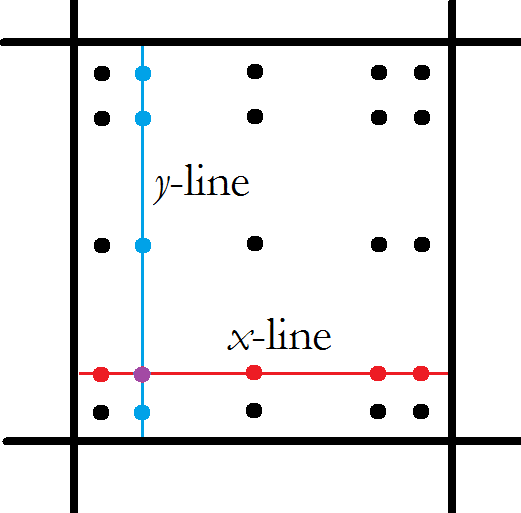
\includegraphics[width=3.5in]{lineDGelemDiag.PNG}
\caption{\label{fig:DGtensorSplit}The splitting of nodal contributions along ``line-wise'' directions on a tensor grid.}
\end{figure}

\be \frac{\partial \omega_{ij}}{\partial t} = (\frac{\partial \omega_{ij}}{\partial t})_{x-line} + (\frac{\partial \omega_{ij}}{\partial t})_{y-line} \ee

%
\section{Flux Interpolation: An Important Distinction}
The flux interpolant can be thought of  as either the interpolation of the product of the velocity and vorticity, or the product of the interpolations of velocity and vorticity; the result of these two interpolants are identical at the nodes
\be I_N f(x_i) = I_N(u(x_i) \omega(x_i)) = I_N(u(x_i)) I_N(\omega(x_i)) \ee
Furthermore, if we perform a Gauss-Legendre quadrature with collocated nodes, the quadrature is exact and the integral of either choice is equal
\be \int f \;dx \approx \sum_i^M u_i \omega_i w_i = \sum_i^M u_i \sum_j^M \omega_j \int \ell_i \ell_j \ee
The interpolation of the product may be order $M$, while the product of the interpolations is order $2M$, but the integral of either is equal; deciding between the two options may appear to be inconsequential. Consider however the case where we wish to integrate the product of the interpolated flux and the derivative of the weighting function. The interpolation of the product is order M and the derivative of the weighting basis M-1, the collocated Gauss-Legendre quadrature is exact

\be \int I_N(f) \, \ell_j'(x) \;dx = \sum_i^M u_i\omega_i \ell_j'(x_i) \ee

There is an important decision that has been implicitly made however. By choosing the quadrature of this form we are choosing the interpolant of the product. The two different flux interpolation choices no longer result in the same integral value. Importantly this means if we expect to need the full interpolatory order N of both the velocity and the vorticity in the stiffness integral, we will not be able to recover them. Instead we will recover the Nth order interpolant of them.

To retain the full order of each quantity, as well as suffer no quadrature error, we would have to instead evaluate the integral of the form
\be \begin{split}\int u(x) \omega(x) \ell_j'(x) \;dx &\approx \int \sum_i^M u_i \ell_i(x) \sum_k^M \omega_k \ell_k(x) \;\ell_j'(x) \;dx\\
&=\sum_i^M u_i \sum_k^M \omega_k \int \ell_i(x) \ell_k(x) \ell_j'(x) \;dx
\end{split}\ee
We will do this in the next section.
%
\section{Modified Quadrature to Retain Interpolation Order (velocity and vorticity)}\label{ModQuad}
To retain full interpolation order of both the velocity and vorticity in the stiffness integral we seek a set of quadrature weights derived from
\be \sum_i^M u_i \sum_k^M \omega_k \;w_{unknown} = \sum_i^M u_i \sum_k^M \omega_k \int \ell_i(x) \ell_k(x) \ell_j'(x) \;dx \ee
note that we might alternatively wish to find something that looks more like the Gauss-Legendre quadrature rule
\be \sum_i^M u_i \sum_k^M \omega_k \sum_q^M \ell_j'(x_q) \;w_{unknown2} \ee
However a better approach is to keep the derivative weighting basis inside the integral.
The derivative of the weighting basis can be derived analytically by use of logarithmic differentiation
\be f' = f \, [ln(f)]' \rightarrow \ell_j'(x)=\ell_j(x) \sum_{\substack{p=0\\ p\neq j}}^M \frac{1}{(x-x_p)} \ee
the resultant form can now be included in the integral.

The integral of the Lagrange basis functions associated with each interpolation times the derivative of the weighting basis must equal the quadrature weight associated that particular integrand, that is rather than M+1  quadrature weights associated with the M+1 nodes of the interpolation of the product, we have the associated $N(M+1)^2$ weights (where N is the number of possible weighting bases, for Galerkin methods N=M of course)
\be \int \ell_i(x) \ell_k(x) \ell_j'(x) \;dx = \mathbf{W}_{ikj} \ee
The integral can be performed numerically using a Gauss quadrature of order at least $3M-1$ to be exact. These weights are pre-calculated at the start of the solver and saved for re-use.

The resultant modified quadrature now takes the form
\ben{modQuad} \int u(x) \omega(x) \ell_j'(x) \;dx \approx \mathbf{u}_i^T \mathbf{W}_{ikj} \, \boldsymbol{\omega}_k \ee
for each $j$th weighting basis function.

This may seem to incur a high cost, until one considers several facts:
\begin{itemize}
\item Normal Gauss-Legendre quadrature requires the stiffness integral be calculated for each weighting basis already, so the $j$ dimension of the quadrature matrix is no worse than before. 
\item One is able to extract \textit{more} information out of the \textit{same} number of interpolation points and achieve superior convergence of the stiffness integral than the standard Gauss-Legendre rule.
\item By including the derivative of the weighting basis in the integral for the quadrature weight matrix, we integrate it exactly a priori. It never appears in the later quadrature of the stiffness integral except implicitly in the quadrature weight matrix itself.
\item The order and definition of the Lagrange basis functions for the vorticity and velocity interpolations are \textit{decoupled}. It is not necessary for the order of the velocity interpolation to be equal to the vorticity. Indeed, the set of interpolation nodes don't even have to be of the same \textit{kind}. It is completely permissible for example to have the vorticity nodes be the Gauss-Legendre nodes, and the velocity nodes to be Lobatto nodes.
\end{itemize}

This has significant advantages for the overall method, both in terms of minimizing both interpolation and quadrature error, as well as giving excellent flexibility in the solver. Normally to vary the order of the velocity interpolation one would need to re-interpolate at the vorticity nodes to recover the flux interpolant. This contributes additional interpolation error, as well as potential aliasing problems. This additional interpolation step would also require about the same number of operations as using the larger quadrature weight matrix, making the two about equal in terms of computational cost. Instead one is free to choose the velocity order freely and the solver adapts seamlessly.

There is an additional computational savings as well. Although we would prefer to use the Legendre points for the vorticity (to preserve the diagonal mass matrix structure that we shall discuss in a coming section), we would like to use Lobatto points for the velocity. Ordinarily we would have to evaluate the boundary velocities and then leave them unused in the stiffness integral with normal Gauss-Legendre quadrature; both the vorticity and velocity would have to share the same  nodes or face re-interpolation costs. This results in wasted velocity evaluations which are the most expensive operation. One might be tempted to only evaluate the velocity at the Legendre points and extrapolate the velocity at the boundaries, but there is no guarantee that the two interpolated velocities from adjacent elements would agree; this would present obvious challenges in the boundary flux evaluation. However by using the modified quadrature matrix one can freely mix node sets, meaning the boundary velocity values are reused in the stiffness integral.

The maximum order polynomial that can be integrated exactly is also similar to some composite quadrature rules (such as Gauss-Kronrod \cite{Roni}); the order depends on whether the number of nodes is odd or even. An even node basis for one of the bases results in a $2M+1$ order accurate method, odd node number results in a $2M$ order accurate method (still sufficient to exactly integrate the product of two Mth order interpolants). A script in Appendix \ref{Algs} validates the convergence claims and order of accuracy of the modified quadrature method.

Table \ref{table:QuadMod} reports an example convergence study for a mixed order/type run with an 7th order Gauss-Legendre and 9th order Gauss-Lobatto quadrature rule showing quadrature error to within machine precision up to order $M+N+1$. It also compares the error in the interpolation of product (IoP) and product of interpolants (PoI), with the latter being an order of magnitude more accurate for this set of example functions.

\begin{table}
\centering
\caption{Convergence of Modified Quadrature for a 7/9th order Method}\label{table:QuadMod}
\begin{tabular}{llllll}
\hline
Order M+N & IoP       & PoI      & Quad. Error & Discretiz. Error &  Order M  \\ \hline
5         & -0.0543   & 0.234    & 2.22e-16         & 0.234                & 3  \\
7         & 0.0162    & 0.0182   & -5.55e-16        & 0.0182               & 4  \\
9         & -0.0143   & 0.0493   & -1.67e-16        & 0.0493               & 5  \\
11        & 0.00342   & 0.00133  & 2.22e-16         & 0.00133              & 6  \\
13        & -0.00182  & 0.00375  & 5.00e-16         & 0.00375              & 7  \\
15        & 0.000445  & 9.38e-05 & 5.55e-16         & 9.38e-05             & 8  \\
17        & -0.000161 & 0.000139 & 8.33e-16         & 0.000139             & 9  \\
19        & 4.20e-05  & 6.15e-06 & 0.000326         & 0.000332             & 10 \\
21        & -1.11e-05 & 2.90e-06 & 0.000523         & 0.000526             & 11 \\
23        & 3.15e-06  & 3.37e-07 & -9.75e-05        & -9.72e-05            & 12 \\ \hline
\end{tabular}
\end{table}

\section{Vortex Dominated Flow: Diagnostics}
Two diagnostics are useful to evaluate the evolution of vortex dominated flows. The first is the vorticity moments of the system, which should be conserved \cite{Koum1997}, and are given by:
\be J_{mn}=\int\int \omega(x,y)x^my^n \; dx\,dy \ee
We shall consider in particular the linear impulse, $J_{01}$ and $J_{10}$.

The other diagnostic considered is the effective aspect ratio \cite{Koum1997}. This is particularly useful when considering the evolution of an elliptical vortex, which will typically undergo some degree of axisymmetrization. The effective aspect ratio is:
\be \lambda_{eff}^2 = \frac{J+R}{J-R} \ee
where $J=J_{20}+J_{02}$, $D=J_{20}-J_{02}$, and $R^2=D^2+4J_{11}^2$.

\section{Discrete $L^2$ error}
The $L^2$ norm is defined as:
\be ||f(x)||_2 = \sqrt{\int f(x)^2 \; dx} \ee
We can use this as a measure of error between two functions:
\be ||u-v||_2 = \sqrt{\int (u-v)^2 \; dx} \ee
A discrete version needs to perform numerical quadrature to calculate the integral of the error. In situations where the calculated error is obtainable at the solution points, we have ready-made quadrature points that we can collocate such that we obtain the discrete form:
\be ||u-v||_2 = \sqrt{[w_i]^T(u_{ij}-v_{ij})^2[w_j]} \ee
where $w_i$ and $w_j$ are the appropriate quadrature weights associated with each direction of the tensor product of quadrature points, and $u_{ij}$ and $v_{ij}$ are the values at the interpolation nodes. If two tests do not share a common set of solution points, we interpolate the results to a shared set of equispaced points and calculate the error by:
\be ||u-v|| =\sqrt{\frac{1}{M\times N} \sum_{i=1}^M \sum_{j=1}^N (u_{ij}-v_{ij})^2 }\ee

%------------------------------------
\chapter{Implementation}
To provide a clear picture of the overarching structure of the solver we restate the overview of \S\ref{Pseudo1}, but now add in specific solver subroutines and more specific details on the required steps.
\section{Overall Solver Structure}
\vspace{-1cm}
\singlespacing
\begin{lstlisting}
Define problem parameters [domain size, initial condition type]
Define solver parameters [order velocity/vorticity, element size,
   time stepping choice, time step, cutoff radius, minimum
   vorticity threshold, kernel type]
Calculate derived solver parameters
   -interpolation nodes/weights
   -modified quadrature matrix
   -node numbering/associativity
   -node coordinates
Setup intitial conditions
Initialize solver
   -vorticity interpolation vectors
   -calculate generalized boundary kernel
   -calculate nearby elemental kernel values
   -calculate quadrature weight outer product for later
      use in pre-multiplication for vorticity integration

for t=0 to end
   if Log?=yes
      save system state to file and plot
   end

   for s=1 to last_stage (NRK14C method)
      Calculate elemental vorticity sums and create mask of
         those greater than threshold
      Pre-multiply vorticity with quad. weight outer product
      
      Calculate un-assigned nearby elemental velocities for
         vorticity source>threshold
      for each vorticity source>threshold
         -Assemble global kernel of boundary values from 
            generalized kernel
         -Calculate global boundary velocities (for surface
            flux use)
         -Correct global boundary values to generate element
            boundary values from far field sources (for
            far field stiffness use)
         -Assign nearby elemental velocities to specific
            element, merge with corrected element boundary
            values for near field sources (for near field
            stiffness use)
      end

      interpolate boundary_vorticity
      calculate numerical_fluxes
      calculate total_surface_flux
      calculate internal_stiffness_flux
		
      vorticity_rate_of_change=...
         internal_stiffness_flux - total_surface_flux
		
      RK_stage= (RK_coeff_a*RK_stage) +...
         (time_step * vorticity_rate_of_change)
      vorticity= vorticity + RK_coeff_b * RK_stage
   end
end
\end{lstlisting}
\doublespacing

We briefly elaborate on the main parts of the implementation, the sections following give full detail for each major part.

We will use terminology commonly used in Finite Element Methods to refer to specific pieces of the 1D PDE solved along each line from Eqn.\,\eqref{DGJoshTemp}; the integral involved in the time derivative generates the \textit{mass} matrix.
\be \boldsymbol{M} = \frac{\Delta x}{2} \sum_{i=0}^M \left[ \frac{d z_{ij}}{dt}	\int_{-1}^{1}\ell_i  \, \ell_j \;dX \right] \ee
The integral involved in the spatial derivative of the weighting function generates the \textit{stiffness} matrix.
\be \boldsymbol{K} = \int_{-1}^{1} f(\aomega) \, \ell_j' \;dX \ee
The total surface flux is the net flow across element bounds into a particular line. It is calculated from the numerical flux and the weighting basis evaluated at the line boundaries.
\be \boldsymbol{F} = \hat{f}\ell_j \Big|^{x_R}_{x_L} \ee

The preamble contains various solver configuration parameters and initializes most of the persistent data objects. It also initializes quadrature information which in turn is used to precalculate the quadrature weight matrices needed for the chosen order of the vorticity and velocity as was described in \S\ref{ModQuad}.

The mass matrix will be shown to be diagonalizable in \S\ref{MassM} allowing it to be decoupled from the time derivative. This allows the quadrature matrix to be multiplied in place to incorporate the Jacobian as well as the inverse Mass matrix entry so that these do not needed to be multiplied by after the fact. 

The next part of the solver creates element-line-boundary-node associativity. These are used to freely select the appropriate sections of data associated with a particular hierarchy. Most of these are simply a column-wise index list, some are specifically shaped so that the returned data from the index selection is the correct shape for reuse (ND matrix etc). This is also where the coordinates of the vorticity nodes, velocity boundary nodes, and velocity internal element nodes are specified. This is more fully described in \S\ref{NodeNum}.

Next, a cell list of functions that specify the initial conditions of the system is evaluated; the initial conditions of the vorticity is the linear sum of each generating function. The resultant initial condition is the linear superposition of all the selected generating functions. The interpolation vectors for the surface flux are constructed, again incorporating the Jacobian and inverse mass entry like in the quadrature weight matrix to avoid element-wise multiplications later. Finally the ``generalized'' and ``nearby'' kernel evaluation matrices are constructed for later re-use as described in \S\ref{VelEval}.

At this point the remainder of the code occurs inside the main time marching loop. A fourth-order, 14 stage, explicit Runge-Kutta routine is used with an inner loop used for stage-stepping. Depending on the solver setup, the velocity evaluation code is either executed every time step, or every stage as described in \S\ref{TimeStep}. The sum of the vorticity in each element is computed and those above a threshold are added to element-wise and line-wise masks. Each element in the mask is treated as a source of vorticity and the velocity from that element is added to the current running total for the global velocity. Total element and element boundary velocities are formed for later use in the semi-discrete system.

The DG advection code always occurs within the RK stage loop. Vorticity is extrapolated at the element boundary. Boundary conditions are applied and the element boundary fluxes are evaluated. The stiffness term is evaluated for the current stage's vorticity and velocity configuration (\S\ref{StiffM}). At this point the semi-discrete system is complete and the stage's rate of change for all nodes is computed for each direction and the two are added together. The new vorticity is computed for the stage and both the time-stepping and stage-stepping loops wrap.

There are also some additional post-processing type routines that run that save simulation data for later use, and can also update in realtime displaying current simulation diagnostics ($L^2$ norm, vorticity conservation etc.).

%
\section{Structured Tensor Mesh}\label{NodeNum}
The test cases that are considered in this thesis are all free of impinging geometry and have no bias known \textit{a priori}, as such a constant-size structured mesh comprised of squares is used. It is worth noting that this is by no means required; an un-structured mesh is easily treated via a mapping to a canonical computational element \cite{Persson2013}. The structured mesh merely affords ease of implementation, as well as simplification of element-line-boundary-node indexing.

Most data is stored in one of two different formats, either a column-major form that matches Matlab's memory layout to optimize indexing performance, or a ``line-wise'' format. The line-wise format groups nodes along the coordinate directions. Adjacent lines are parallel 1D basis functions that share a boundary node. Lines are numbered left to right, bottom to top for $x$-lines and bottom to top, left to right for $y$-streams. Both direction's lines are numbered separately. For an example layout of $x$ and $y$ lines see Figure~\ref{fig:streams}. The inset only shows the upper left segment of a 5x4 global domain. The lowest two $y$-lines shown aren't sequential because one needs to continue counting in the $y$ direction from 1, there are 3 more elements with the left most $y$-line in each numbered '2,3,4' sequentially. Once we reach the top of the global domain the numbering wraps back around to the bottom, second leftmost $y$-stream: '5'.

\begin{figure}
\centering
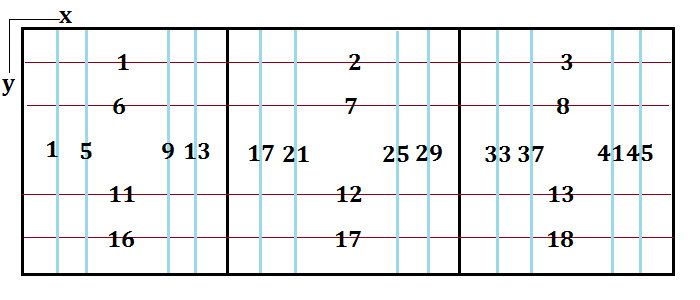
\includegraphics[width=6in]{streams.PNG}
\caption{\label{fig:streams}``Line-wise'' numbering for elements 1, 5, and 9 in a 5x4 element global domain.}
\end{figure}

%
\section{Boundary Conditions}
In a finite element method, natural boundary conditions are typically handled automatically. The global domain of the model is sized so that no vorticity is advected past the boundary. Should vorticity still manage to pass the boundary it will be lost due to a 'NoInflow' condition; this is imposed by enforcing all surface flux along the domain boundary to be 0. Any vorticity that does reach the boundary is destroyed.

A set of periodic boundary conditions were also created that permit study of toroidal or infinite cylinder domains that may be useful in the study of semi-infinite phenomena such as the Kelvin-Helmholtz instability on a infinite line of vorticity.

%
\section{Mass Matrix}\label{MassM}
As discussed in \S\ref{INC}, the set of Legendre roots for the vorticity interpolation points results in
\be \int \ell_i(x) \ell_j(x) dx = \delta_{ij} w_j \ee
This proves particular useful for the mass term, meaning the choice of Legendre nodes for interpolation results in a diagonal mass matrix that is trivially invertible.  Eqn.\,\eqref{DGJoshTemp} is then simplified to
\ben{DGJoshTemp2} \frac{d \aomega_j}{dt} \frac{w_j \Delta x}{2}
+\hat{f}\ell_j \Big|^{x_R}_{x_L} 
- \int_{-1}^{1} f(\aomega) \, \ell_j' \;dX = 0 \ee

One could instead choose the set of Lobatto points to avoid extrapolating the vorticity at the element boundaries, but this would result in a full mass matrix that when inverted necessitates a matrix-vector product which is about as computationally expensive as extrapolating the boundary vorticity.

%
\section{Stiffness Matrix}\label{StiffM}

\begin{figure}
\centering
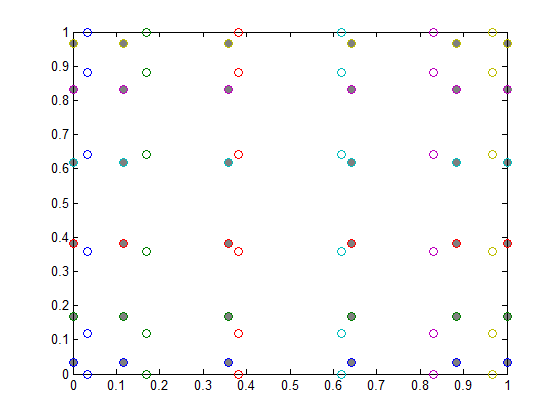
\includegraphics[width=5.5in]{VelocityLobatto.PNG}
\caption{\label{fig:VelocityLobatto}5$^{th}$ order Lobatto velocity nodes along $x$-lines (dark circles) and $y$-lines (empty circles).}
\end{figure}

We can apply the results for the modified quadrature rule from Eqn.\,\eqref{modQuad} to the purpose of evaluating the stiffness integral we have left unevaluated thus far. Recall that for maximum flexibility the velocity interpolation order is independent of the vorticity order. In addition the Lobatto points are chosen for the velocity to reuse the boundary velocities. At first glance it might seem actually counter productive to choose a different order or set of nodes for the velocity. To avoid needing ``off-line'' interpolation the velocity nodes should be co-linear with the vorticity lines. The result for a 5th order velocity and vorticity field is shown in Figure~\ref{fig:VelocityLobatto}.

It would appear we actually need double the velocity evaluation points. The non-square tensor product of the Lobatto nodes with the Legendre nodes means that the $x$-line velocity nodes will never coincide with the $y$-line velocity nodes. The solution to this is that the velocity is evaluated in a component-wise manner. Along the $x$-line we only require $u_x$ and along the $y$-line we only require $u_y$. The different direction's line's nodes may not coincide with each other, however this doesn't pose any problems as we do not need need the other velocity component at any particular velocity node. A small caveat is that if we would like to calculate the full velocity field this must be added in as an additional post-processing step to calculate the skipped velocity components.

We can now apply the modified quadrature matrix to our elemental PDE
\ben{DGJoshTemp3} \frac{d \aomega_j}{dt} \frac{w_j \Delta x}{2}
+\hat{f}\ell_j \Big|^{x_R}_{x_L} 
- \mathbf{u}^T \mathbf{W}_{--j} \, \boldsymbol{\omega} = 0 \ee
rearranging to obtain the rate of change of the nodal vorticity
\ben{DGJosh} \frac{d \aomega_j}{dt}
=\frac{2}{w_j \Delta x} \left[\mathbf{u}^T \mathbf{W}_{--j} \, \boldsymbol{\omega} - \hat{f}\ell_j \Big|^{x_R}_{x_L}\right]  \ee
This nodal equation now describes the line's contribution to the time evolution of a particular node. This calculation is performed for all vorticity nodes on all $x$-lines and added to the rate of change of the matching vorticity nodes in the $y$-lines.

%
\section{Velocity Evaluation}\label{VelEval}
It is important to note that direct pair-pair velocity evaluation has $\mathcal{O}(N^2)$ complexity; it is well known that methods exist that can reduce this to $\mathcal{O}(N\text{log}N)$ or even $\mathcal{O}(N)$ \cite{SchumannSweet1976,LindsayKrasny2001,BarnesHut1986,GreengardRokhlin1987}. However for ease of implementation and to eliminate the effects of as much approximation error as possible on validation, the velocity is evaluated directly at each desired velocity point by means of the desingularized Biot-Savart integral (Eqn.\,\eqref{DesingBS}). 

The velocity at a particular node is calculated by summing the net effect of each masked source element. A loop steps through each source element and adds it's contribution to all velocity nodes. The Biot-Savart integral is done via a 2D tensor product Gauss-Legendre quadrature of order equal to the vorticity field with quadrature points collocated at the vorticity interpolation points. 
\be u(x^*)= \sum_{E=1}^{N_{mask}} [\omega_{pre}]^TK_{\delta}(x^*-[x_E]) \ee
\be \omega_{pre} = [\omega(x_E)].*[w_i \otimes w_j]\ee
Items in brackets are column vectors and $.*$ indicates element-wise multiplication. $\omega_{pre}$ is the vorticity for each element in the mask pre-multiplied by the outer product of the two tensor direction's 1D quadrature weights. As a given mask element appears as a source for all velocity evaluation points, performing the multiplication by the quadrature weights and caching realizes significant savings. This technique combined with the summation of all quadrature points in a  particular source element by a vector-vector product realizes a significant speed-up: over 2000\% over the more natural but slower vector-(matrix-matrix)-vector multiplication, $[w_i]^T(\omega.*K_{\delta})[w_j]$.

\begin{figure}
\centering
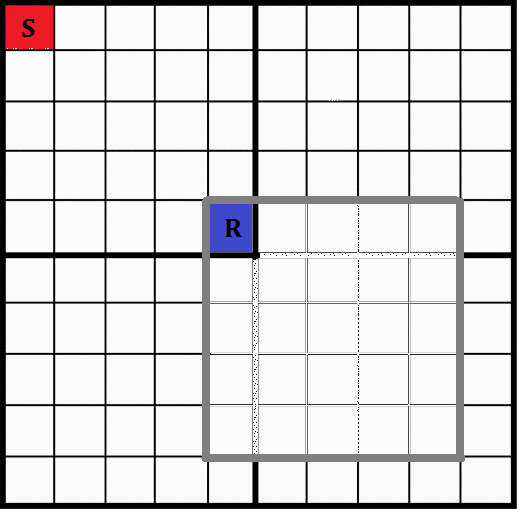
\includegraphics[width=5.5in]{GlobalKernel.PNG}
\caption{\label{fig:GlobalKernel}The ``global'' kernel matrix showing (R)eference source and actual (S)ource, the upper left quadrant is the actual full domain, the selected region with respect to (R) selects the correct values of the kernel for (S).}
\end{figure}

\subsection{Biot-Savart Kernel Calculations}
The majority of the cost of the present solver results from the assembly of the boundary kernel values from the generalized template. One is presented with three options: calculate a new set of kernel values for each source element, form a ``global'' matrix of kernel values that one maps to the particular source element under consideration, or directly calculating and storing kernel values for every source-node pair.

The first choice is the most direct, but also the slowest. It is bottlenecked by computational cost; the number of operations to form the kernel actually exceeds those needed to evaluate the integral. The third method is the fastest, but bound by memory constraints which scale as $Np^4 K^4$. Even a modest 5th order velocity method with 20x20 elements (~15k degrees of freedom) would require 1.66GB of memory to store: kernel values per target node x number of targets = $[30^2(6^2)][30^2(6^2)]\times$8bytes/double float .

The second method is the one currently used in the code. The global domain is reflected about both axes for a central element and the kernel values are calculated for all elements in relation to the reference source. Depending on where the actual source element is in the true domain determines what portion of the global domain is selected with respect to the reference element, see Figure~\ref{fig:GlobalKernel}. This is implemented in the solver as

\singlespacing
\begin{lstlisting}[language=Matlab]
kernel_xB= ...
   gkernel_xB(:, [1:Np*K(2)] +Np*(K(2)-Enum_y(Src)),...
   [1:K(1)+1] +(K(1)-Enum_x(Src)) );
kernel_yB=...
    gkernel_yB(:, [1:Np*K(1)] +Np*(K(1)-Enum_x(Src)),...
   [1:K(2)+1] +(K(2)-Enum_y(Src)) );
\end{lstlisting}
\doublespacing

where K(x,y) is the number of elements, Np is the number of interpolation points along one direction, Enumx/Enumy return the x and y directional numbering of Src (the global element number), and gkernel\_xB/gkernel\_yB is the generalized kernel values that contain x and y reflections of the domain.

This realizes significant computational savings from not having to repeatedly recalculate the kernel values, however it is memory access bottlenecked. Repeatedly selecting and manipulating non-contiguous blocks of memory accounts for about 60\% of CPU time according to the profiler. Even being careful to arrange as much data column-major as possible only delays the problem.

This also means otherwise ``empty'' elements affect performance by further fragmenting the global kernel matrix. At some point the sparseness of the domain is sufficient that the recalculation of the kernel for each source outperforms an overly fragmented global matrix. Note that the memory bottleneck limitation is not an intrinsic property of the underlying method itself, but rather a consequence of the solver implementation and Matlab's underlying memory model.

\subsection{Convergence}
For the far field canonical Gauss-Legendre quadrature performs as expected, with excellent convergence. However for elements directly neighboring the source element, as well as the source element itself, the nearly singular nature of the integral poses convergence problems for the quadrature \cite{Strain1996}. As an illustrating point consider the data in Tables \ref{table:SelfBSQuad} and \ref{table:2BSQuad}. Compare the relative error for the computed velocities due to self-influence and a source element just two elements away. The difference in the relative error is approximately 5 orders of magnitude. Furthermore the observed error in the two element away case is mostly discretization error: the same integration parameters performed with a dummy kernel of $K=1$ had a relative error of 5E-10, within an order of magnitude of the actual test case.

\begin{table}
\centering
\caption{Relative error in computed velocities for the self-influence of an element; 5th order quadrature method for a Gaussian vorticity distribution, $K_{WL}$, $\delta=0.35h$}\label{table:SelfBSQuad}
\begin{tabular}{l|lllllll}
       &$ LGL(x_1)$             &$ LGL(x_2)$              &$ LGL(x_3)$              &$ LGL(x_4)$             &$ LGL(x_5)$              & $LGL(x_6)$            \\ \hline
$GL(x_1)$ & 0.0014 & 0.0028 & 0.0047  & 0.0011 & 0.00011 & 0.00012\\
$GL(x_2)$ & 0.0012 & 0.00096 & 0.0011  & 0.0022 & 9.4e-06 & 0.00016 \\
$GL(x_3)$ & 0.0014 & 0.0051  & 0.0024  & 0.0060 & 0.0037  & 0.00030 \\
$GL(x_4)$ & 0.0010 & 0.0023  & 0.0018 & 0.0047 & 0.0062  & 0.00037 \\
$GL(x_5)$& 0.0021 & 0.0021  & 0.0042  & 0.0060& 0.0081  & 0.00018 \\
$GL(x_6) $& 0.0016 & 0.0042 & 0.00024 & 0.0067 & 0.0035  & 0.00028
\end{tabular}
\end{table}

\begin{table}
\centering
\caption{Relative error in computed velocities for an element two elements away from the source; 5th order quadrature method for a Gaussian vorticity distribution, $K_{WL}$, $\delta=0.35h$}\label{table:2BSQuad}
\begin{tabular}{l|lllllll}
       &$ LGL(x_1)$             &$ LGL(x_2)$              &$ LGL(x_3)$              &$ LGL(x_4)$             &$ LGL(x_5)$              & $LGL(x_6)$            \\ \hline
$GL(x_1)$ & 7.67E-09 & 6.79E-09 & 5.88E-09 & 1.85E-09 & 2.49E-09 & 4.38E-09 \\
$GL(x_2)$    & 9.87E-09 & 9.28E-09 & 8.13E-09 & 2.56E-09 & 3.39E-09 & 5.91E-09 \\
$GL(x_3)$   & 1.49E-08 & 1.51E-08 & 1.35E-08 & 4.00E-09 & 5.95E-09 & 9.95E-09 \\
$GL(x_4)$    & 2.42E-08 & 2.79E-08 & 2.42E-08 & 6.16E-09 & 1.22E-08 & 1.91E-08 \\
$GL(x_5)$    & 3.79E-08 & 4.58E-08 & 4.16E-08 & 8.24E-09 & 2.45E-08 & 3.55E-08 \\
$GL(x_6)$    & 5.08E-08 & 6.38E-08 & 5.97E-08 & 9.02E-09 & 3.92E-08 & 5.40E-08
\end{tabular}
\end{table}

The weighting function for the Legendre polynomials is simply $w_{Leg}(x)=1$. As such, the product of the $K_{\delta}$ and the vorticity near the source element is poorly interpolated by a polynomial. To illustrate consider the same setup as the one used in the tabulated velocity errors comparison: plots of the true product of the vorticity and $K_{WL}$, it's matching interpolation, and the error between them are plotted in Figures \ref{fig:wKtrue}, \ref{fig:wKinterp}, \ref{fig:wKerror} respectively.

\begin{figure}
\centering
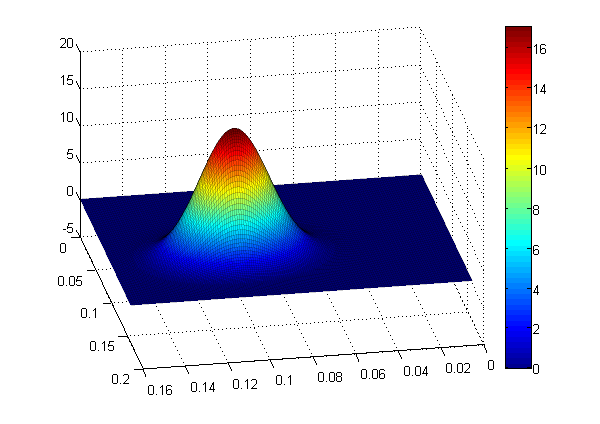
\includegraphics[width=5.5in]{wKtrue.PNG}
\caption{\label{fig:wKtrue}True product of example $\omega$ and $K_{\delta}$.}
\end{figure}
\begin{figure}
\centering
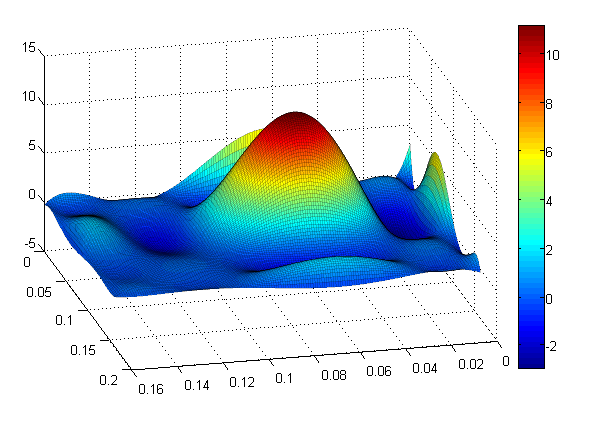
\includegraphics[width=5.5in]{wKinterp.PNG}
\caption{\label{fig:wKinterp}Interpolated product of example $\omega$ and $K_{\delta}$.}
\end{figure}
\begin{figure}
\centering
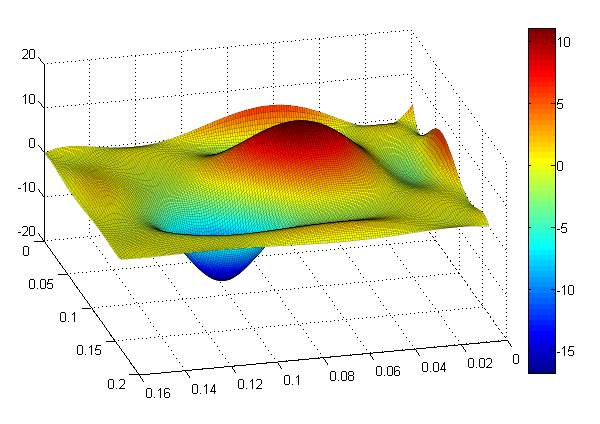
\includegraphics[width=5.5in]{wKerror.PNG}
\caption{\label{fig:wKerror}Error between true and interpolated products.}
\end{figure}

Ideally one would use a weighting function of a form similar to the singular portion of the kernel to form a new orthogonal basis, but here one is limited by the tensor basis. More freedom is required in the interpolation points to provide adequate leeway to generate desirable quadrature rules. The generation of general multivariable interpolation and quadrature bases is an area of active and relatively recent effort \cite{Gasca2000,Xu2012,Gautschi2013}.

%
\section{Vorticity Sparseness}
One of the advantages of DG as an advection scheme is the compact local support. This means that for a large domain with only sparse vorticity one should be able to only consider those elements that contain vorticity. The sparseness can be applied in several ways. From the DG perspective, if an element is empty than there is nothing to advect and the element can be omitted from the evaluation entirely. The reality is that even small numerical errors in the boundary flux may lead to non-physical perturbations in the vorticity field in what should be otherwise empty elements. These elements can no longer be ignored, lest some instability result from improperly handling non-zero elements.

From a vorticity-velocity perspective elements with zero vorticity or boundary flux driven ``noise'' are unimportant, even if they are important from a consistency standpoint for the DG part of the code. Therefore a threshold value can be specified, elements with total vorticity less that the threshold value are ignored, and only those elements above the threshold are put in a mask. The masked elements are the ones considered as sources for the velocity evaluation. Additionally, only the boundary velocities for these unimportant elements are calculated and a reduced velocity order stiffness term is calculated for them.

The current state of the solver is bottlenecked by the velocity evaluation, so although some savings would be realized by maintaining true vorticity domain sparseness, the result is that it has little impact on the overall solution time. The unmasked elements have only a marginal impact on the cost of the velocity evaluations.

%
\section{Explicit Time-Stepping}\label{TimeStep}
With the semi-discrete system formed, one must now select a time discretization scheme. For simplicity an explicit time-stepping method will be used. The diagonalized mass matrix created in \S\ref{MassM} permits the compact rearrangement of Eqn.\,\eqref{DGJoshTemp2} to solve explicitly for the nodal rate of change of vorticity due to each of the lines that intersect the node. The contribution from each line is added and the total rate of change is used to advance stagewise within the RK routine:

\singlespacing
\begin{lstlisting}
for t=0:delt:EndTime %Step
    for i=1:nS %Stage
        (Velocity calculations)
        (semi-discrete calculations for advection)
        wx_dt= permute(Stiff_x-SurfFlux_x,[4 1 3 2]);
        wy_dt= reshape(reshape(...
	Stiff_y-SurfFlux_y,K(2),[])',Np,1,[]);
        
        k2= RKa(i)*k2 + delt*(wx_dt+wy_dt);
        wx= wx+RKb(i)*k2;
        wy= reshape(reshape(wx,K(1)*Np,[])',Np,1,[]);
    end
end
\end{lstlisting}
\doublespacing

where $delt$ is the timestep, $nS$ is the number of stage RK method chosen, $RKa$ and $RKb$ are RK specific coefficients, $Stiff\_x$/$Stiff\_y$ are the nodal stiffness values, $SurfFlux\_x$/$SurfFlux\_y$ are the nodal surface flux values, $k2$ is the low-storage RK state variable, and $wx$/$wy$ are line-wise vorticity state variables

The two chief categories are multi-step and multi-stage methods, typically either Adams-Bashforth or Runge-Kutta respectively \cite{ButcherSurvey}. It is known that Forward Euler and AB2 are unstable for DG with an upwind flux due to it's dissipative nature \cite{Reid}. The choices permitted then are Runge-Kutta or a higher-order Adams-Bashforth.

The recent thesis work of Atcheson \cite{Reid} presents a comprehensive overview of the optimal choice of time-stepping algorithm for a DG operator. In particular it was shown that Runge-Kutta methods outperformed AB3 and that all higher-order Adams-Bashforth schemes required far too restrictive of a time-step to satisfy the CFL condition to be efficient. Out of all the Runge-Kutta schemes considered \cite{Toulorge} one of the more competitive options was the ``NRK14C'' scheme developed by Niegemann et al. \cite{Niegemann}. This is an optimized 4th order, 14 stage low storage scheme of similar structure to other 2N style schemes \cite{Carpenter}.

Notably, NRK14C permits a time-step 1.86 times as long per stage than the canonical RK4 assuming the limitation is the negative real component in the stability region of the method. This equates to a proportional runtime decrease for almost negligible implementation effort. 

There is one further choice to be made regarding time-stepping: where to include the velocity evaluation. It is reasonable to assume that in practice the numerical stiffness of the problem is due to the DG operator, not the velocity evaluation. This means one is free to either evaluate the velocity at each stage, or instead to evaluate at the start of each step. 

Of course the time discretization error of the velocity field will be increased, but the runtime of the resultant method will be an order of magnitude faster. If the CFL condition is stringent enough to necessitate a small time-step compared to the evolution rate of the velocity, the velocity evaluation is moved outside of the stage loop. The effect on the overall convergence of the method is important to consider when making this choice.

%------------------------------------
\chapter{Results}
\section{Validating Test Cases}
Of primary interest in the development of a new method is validation with common test cases, as well as an evaluation of convergence. The following test cases are evaluated and examined for a range of items of interest: behavior of Biot-Savart kernel choice and cutoff radius, stage vs step-wise velocity evaluation, effect of velocity order, convergence rate of vorticity and velocity, $L^2$ error, and appropriate conservation of vorticity and linear impulse.

\subsection{Perlmann: Stationary Vortex}
Perlmann's 7th order polynomial was the first case studied \cite{Perlmann1985}. The intial condition is a stationary vortex that permits an analytical solution to compare against. The initial vorticity distribution is of the form:
\ben{PerlW} \omega(z)=(1-|z|^2)^7, \; |z|\leq 1  \quad \omega(z)=0, \;|z|>1 \quad z^2=x^2+y^2 \ee
and the corresponding velocity field is:
\ben{PerlU} u(z,t)=f(|z|)\binom{y}{-x} \ee
where
\[
f(|z|)=
\begin{cases}
    -\frac{1}{16|z|^2}(1-(1-|z|^2)^8)	& |z| \leq 1\\
    -\frac{1}{16|z|^2} 			& |z|>1
\end{cases}
\]
and are invariant with time. This test case is particularly useful as the availability of an analytical solution allows an accurate assessment of the $L^2$ error of the computed solution. Having an analytical solution also permits the full investigation of various methodology choices; a range of combinations of method parameters can be experimented with to empirically select reasonable choices for the de-singularized Biot-Savart kernel type, cutoff radius, stage vs stepwise velocity evaluation, and the approximation order of the velocity with respect to the vorticity approximation order.

\subsection{Strain: Interacting Vortex Patches}
Strain's system of interacting random vortex patches \cite{Strain1996} forms the next validation case. Specific initial conditions are specified for each of the vortex patches in Table \ref{table:StrainTable} with the overall system consisting of the linear superposition of each patch
\ben{StrainV} \omega(x,y,0) = \sum_{j=1}^m \Omega_j exp(-((x-x_j)^2 + (y-y_j)^2)/\rho_j^2) \ee
An explicit data set for the results is not reported, but a set of contour plots illustrates the time evolution. The same parameters are used in the present solver and similar contour plots are compared against the validating set.

This test case has several features that make it a useful diagnostic test. The relative motion of each vortex is important in this case to compute an accurate solution, both short and long-range interactions need to be accurately computed. Additionally the onset of a vortex collision occurs, creating strong vorticity gradients which are more difficult to discretize.

\begin{table}
\centering
\caption{Interacting Vortex Patch Parameters}\label{table:StrainTable}
\begin{tabular}{lllll}
\hline
j & $x_j$    & $y_j$    & $\rho_j$ & $\Omega_j$ \\ \hline
1 & -0.6988 & -1.7756 & 0.6768  & -0.4515   \\
2 & 1.4363  & -1.4566 & 0.3294  & 0.4968    \\
3 & -0.1722 & 0.4175  & 0.5807  & -0.9643   \\
4 & -1.5009 & -0.0937 & 0.2504  &  0.3418    \\ \hline
\end{tabular}
\end{table}

\subsection{Koumoutsakos: Elliptical Vortex}
The final validation case is the evolution of an elliptical vortex patch \cite{Koum1997}. The specific initial configuration is specified as
\be \omega^{II}(r) = 20(1-(r/0.8)^4), \; r\leq 0.8 \quad \omega^{II}(r)=0, \; r>0.8 \ee
however the cases tested were actually elliptical, to accommodate this the initial distribution was modified to
\ben{KoumEqn} \omega^{II}(x,y,0)_{mod} = 20(1-((x/a)^2+(y/b)^2)^2/0.8^4 ) \quad a=1, \; b=2 \ee
The contour levels are specified in the resultant figure as 0.25, 0.50, 1, 2, ..., 20; these levels are used in the current code's resultant plot for direct comparison.

This test case also has several relevant diagnostic features. The elliptical distribution of the vortex rotates creates weak filamentary structures that are important to properly resolve and accurately advect as they later collide with the main vortex body. Additionally, the initial profile of the vortex has no continuous derivatives at the transition from the vortex core to the surrounding fluid which provides a challenging test for the polynomial basis functions.

%%
\section{Perlmann: Stationary Vortex}
Unless otherwise specified, all experiments are stage-wise velocity evaluation with a time step of 0.5 seconds.
\subsection{Comparison of Biot-Savart Kernel Effects}\label{Pkern}
The first method choice examined is the de-singularized Biot-Savart kernel, with Eqns.\,\eqref{RMkern}, \eqref{SGkern}, \eqref{PSkern0}, and \eqref{PSkern2} tested. It is important to determine the kernel's effect on the order of convergence of the vorticity and velocity. Figures \ref{fig:KernW} and \ref{fig:KernU} plot the convergence of the vorticity and velocity respectively for the Rosenhead-Moore, Winckelmans-Leonard, and Spectral kernels. Solver parameters were chosen to obtain the minimum $L^2$ norm of the vorticity at the end of 20 seconds (the time period studied by \cite{Perlmann1985}) for a 6th order method. In all of the exploratory runs the spectral desingularized Biot-Savart kernels were found to give the best combination of $L^2$ norm, rate of convergence, and the additional convenience of not requiring changing depending on the order of the method and will be used henceforth unless otherwise specified.
\begin{figure}
\centering
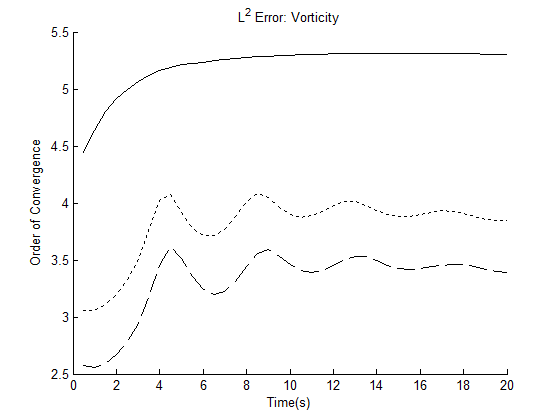
\includegraphics[width=1\textwidth]{KernW.PNG}
\caption{\label{fig:KernW}Comparison of convergence effects on vorticity by kernel for Spectral(-), WL(..), and RM(- -) kernels, 6th order method.}
\end{figure}
\begin{figure}
\centering
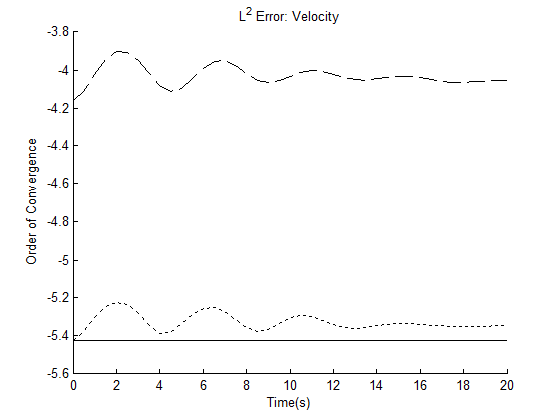
\includegraphics[width=1\textwidth]{KernU.PNG}
\caption{\label{fig:KernU}Comparison of convergence effects on velocity by kernel for Spectral(-), WL(..), and RM(- -) kernels, 6th order method.}
\end{figure}

%
\subsection{Cutoff Radius Effects}\label{Pcutoff}
The cutoff radius is an important parameter in the desingularization of the Biot-Savart kernel. If it is too large it unnecessarily smooths the flow and the approximation error is larger with no added benefit. If it is too small the kernel is too close to singular and the quadrature error will be large. A proper cutoff radius choice will balance the two errors so they are of the same magnitude to minimize the total overall error. Figure \ref{fig:CutoffW} and \ref{fig:CutoffU} compare the $L^2$ errors for the vorticity and velocity respectively for a 6th order method. The cutoff radius is allowed to vary according to mesh size such that $\delta/\Delta x$ remains constant for a particular fixed order. Solver parameters were chosen to be the same as spectral kernel experiment used in \S \ref{Pkern}.

Figure \ref{fig:CutoffL2} plots the log of the $L^2$ error for cutoff radii with similar rates of convergence for velocity, one with too small and the other too large of a cutoff radius to properly discriminate the difference in time varying behavior of the convergence rate for vorticity for these cutoff radii. Despite them having similar rates of convergence, the $L^2$ error is much smaller in the one with $\delta=0.1/\Delta x$ For this one the rate of convergence of vorticity is actually greater initially than all others, but decays as the solution evolves.

\begin{figure}
\centering
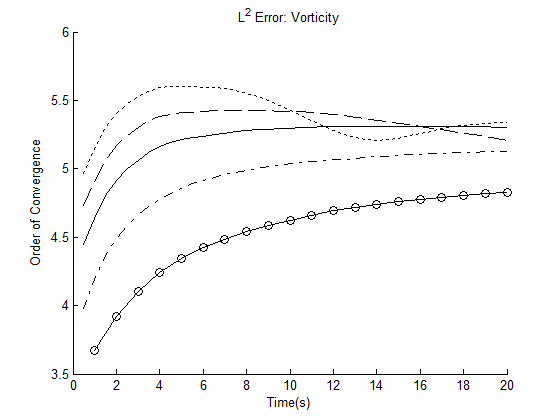
\includegraphics[width=1\textwidth]{CutoffW.PNG}
\caption{\label{fig:CutoffW}Comparison of convergence effects on vorticity by cutoff radius for $\delta/\Delta x$=0.1(..), 0.2(- -), 0.3(-), 0.5(-.), 0.9(-o).}
\end{figure}
\begin{figure}
\centering
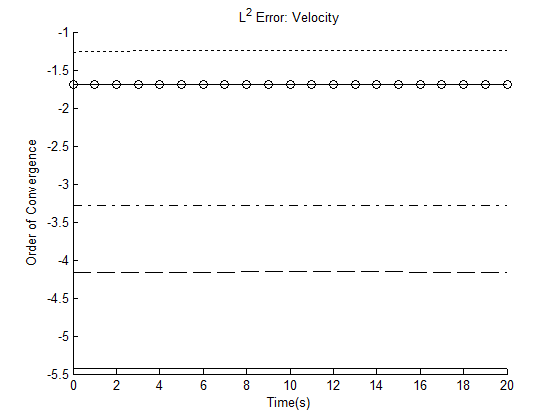
\includegraphics[width=1\textwidth]{CutoffU.PNG}
\caption{\label{fig:CutoffU}Comparison of convergence effects on velocity by cutoff radius for $\delta/\Delta x$=0.1(..), 0.2(- -), 0.3(-), 0.5(-.), 0.9(-o).}
\end{figure}
\begin{figure}
\centering
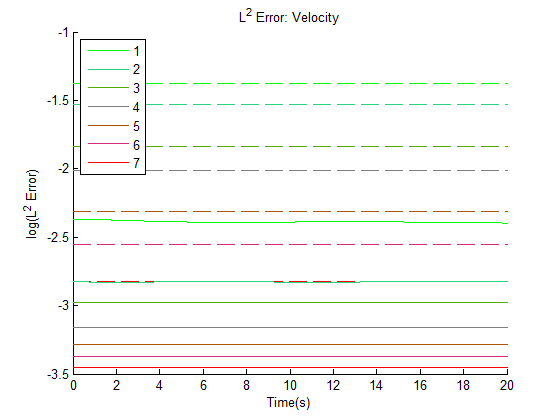
\includegraphics[width=1\textwidth]{CutoffL2.PNG}
\caption{\label{fig:CutoffL2}Comparison of log $L^2$ error on velocity by cutoff radius for $\delta/\Delta x$=0.1(-) and 0.9(- -).}
\end{figure}
%
\subsection{Stage vs. Step-wise Velocity Evaluation}
A sixth order method with $\delta=0.3$ was used to compare stage vs. step-wise evaluation of the velocity. Solver parameters were otherwise identical to the matching cutoff radius test in \S\ref{Pcutoff} with $7^2$ elements. Figure \ref{fig:StageVSStep} plots a comparison of the two choices with identical time-step. The resulting $L^2$ error in vorticity is identical between the two choices, with no discernible difference apparent in the plot. Although there appears to be no difference, stage-wise velocity evaluation will continue to be used unless specified otherwise until it is retested for a problem other than a stationary vortex.

\begin{figure}
\centering
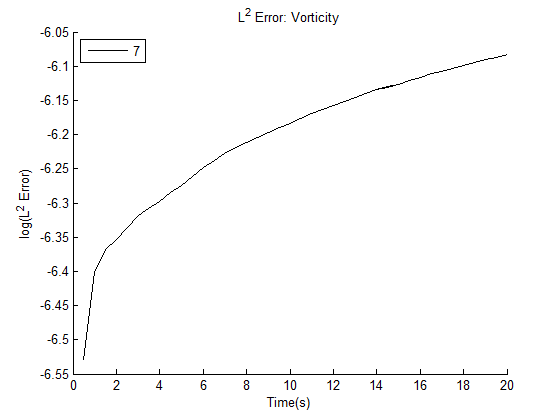
\includegraphics[width=1\textwidth]{StageVSStep.PNG}
\caption{\label{fig:StageVSStep}Comparison of stage-wise(-) and step-wise(- -) evaluation of velocity, with indiscernible difference between the two.}
\end{figure}

%
\subsection{Minimum Order Velocity Required to Maintain Overall Order of Convergence}
The method permits the order of the velocity polynomial basis to be varied independently from the vorticity basis thanks to the modified stiffness quadrature method described in \S \ref{ModQuad}. If one were able to achieve comparably accurate solutions with a lower order velocity field significant savings could be realized.

Figure \ref{fig:VariableUWL2} plots the $L^2$ error of the vorticity for a 6th order method with a 2nd through 7th order velocity field. Figure \ref{fig:VariableUWConvergence} plots the convergence of the various order velocity tests. The 6th and 7th order velocity solutions have nearly identical convergence rates. In general the convergence rate is one half order less than the order of velocity field, but is ultimately limited by the order of the vorticity; the 7th order velocity field solution converges at the same rate as the 6th order velocity solution.

\begin{figure}
\centering
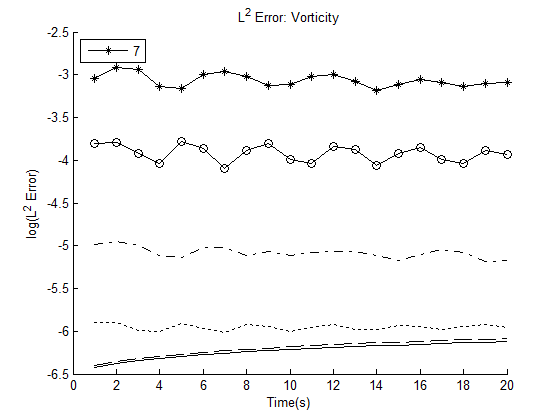
\includegraphics[width=1\textwidth]{VariableUWL2.PNG}
\caption{\label{fig:VariableUWL2}$L^2$ error in vorticity for velocity order: 2(-*), 3(-o), 4(-.), 5(..), 6(- -), and 7(-).}
\end{figure}
\begin{figure}
\centering
\includegraphics[width=1\textwidth]{VariableUWConvergence.PNG}
\caption{\label{fig:VariableUWConvergence}Comparison of convergence rate for reduced velocity order experiment, velocity order: 2(-o), 3(-.), 4(..), 5(- -), 6/7(-).}
\end{figure}

%
\subsection{Convergence Rates of Various Orders}
All previous experiments were performed with a sixth order method to allow room for degradation of the observed convergence rate. They have established reasonable choices for kernel type, cutoff radius, stage-wise velocity evaluation, and setting the order of the velocity field equal to the vorticity field. We can now assess the overall behavior with respect to the order of the vorticity field, keeping all solver parameters set to values appropriate for the respective vorticity order.

A 3rd through 6th order method was used to measure convergence rate; the 6th order method has identical solver parameters as that used in the previous experiments. Figure \ref{fig:Porder} provides a comparison of the observed convergence rate of the vorticity for each of the various order methods. The 3rd and 4th order methods converge at full order, while the 5th and 6th order solutions converge at a little more than one half of an order less than optimal.

\begin{figure}
\centering
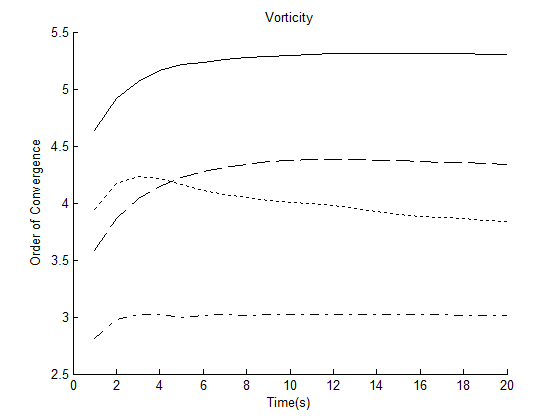
\includegraphics[width=1\textwidth]{Porder.PNG}
\caption{\label{fig:Porder}Comparison of convergence rate for various order methods: 3rd(-.), 4th(..), 5th(- -), and 6th(-).}
\end{figure}

There is an additional benefit to using a higher-order method beyond a greater convergence rate. Even for solutions with a similar number of degrees of freedom the resultant $L^2$ error in the vorticity is lower with a higher order method. Figure \ref{fig:PL2} compares the the $L^2$ error in vorticity for 3rd through 6th order methods employing various numbers of elements to achieve approximately 2500 degrees of freedom. The sixth order method's error is two orders of magnitude lower than the 3rd order method, a significant improvement.

\begin{figure}
\centering
\includegraphics[width=1\textwidth]{Pl2.PNG}
\caption{\label{fig:PL2}Comparison of $L^2$ errors for various order methods with a fixed number of degrees of freedom: 3rd(-.), 4th(..), 5th(- -), and 6th(-).}
\end{figure}

%
\subsection{Conservation of Vorticity}\label{PConserveW}
One of the main advantages of the velocity-vorticity is explicit conservation of vorticity. Figure \ref{fig:PWconserve} plots the log of relative conservation of vorticity with respect to initial total vorticity at t=0. At later times in each solution the conservation of vorticity generally improves, more so for solutions with few elements. Figure \ref{fig:PWconserveConverge} plots the rate of convergence of conservation of vorticity for these solutions. The rate of convergence decays at later times as a result of the lower element number solutions benefiting more from the gradual improvement of conservation of vorticity over time and is not necessarily indicative of the rate of convergence of the overall problem.

\begin{figure}
\centering
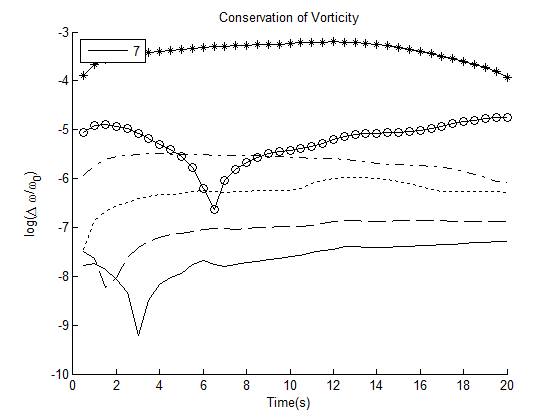
\includegraphics[width=1\textwidth]{PWconserve.PNG}
\caption{\label{fig:PWconserve}Conservation of vorticity in a 6th order method, K$\times$K elements: K=2(-*), 3(-o), 4(-.), 5(..), 6(- -), and 7(-).}
\end{figure}
\begin{figure}
\centering
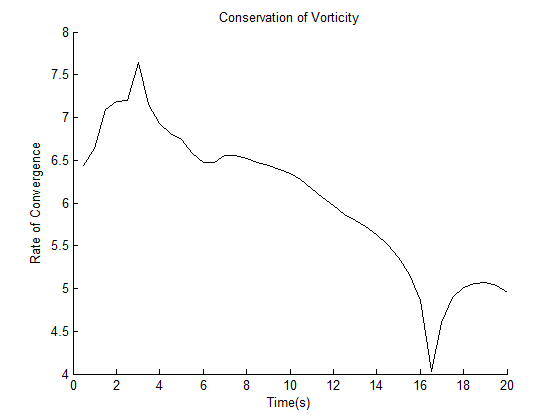
\includegraphics[width=1\textwidth]{PWconserveConverge.PNG}
\caption{\label{fig:PWconserveConverge}Convergence rate of conservation of vorticity, sixth order method.}
\end{figure}
%
\subsection{Conservation of Linear Impulse}
Similar to total vorticity, moments of vorticity should also be conserved. The first moment, linear impulse can provide a useful diagnostic to check the validity of the solution. Figure \ref{fig:PLinImp} plots the total linear impulse for the sixth order method with varying numbers of elements. It is conserved to within nearly machine precision; solutions with more elements actually display a decrease in conservation of linear impulse, which is likely a result of a higher rate of accumulation of roundoff errors due to the greater number of degrees of freedom.
\begin{figure}
\centering
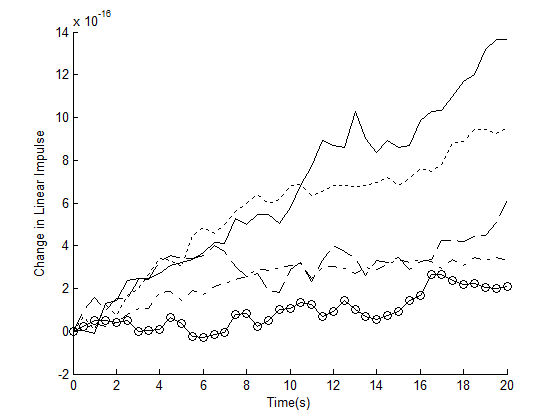
\includegraphics[width=1\textwidth]{PLinImp.PNG}
\caption{\label{fig:PLinImp}Conservation of linear impulse, sixth order method with K$\times$K elements K= 3(-o), 4(-.), 5(..), 6(- -), and 7(-).}
\end{figure}

%%
\section{Strain: Interacting Vortex Patches}
With convergence established for the overall method a more challenging system will be examined.
%
\subsection{Comparison with Originally Published Results}\label{SComp}
Although an analytical solution does not exist for the given vortex system, we shall compare the solution from the present method with that obtained by Strain in \cite{Strain1996}. He does not note the contour intervals used in the creation of his plots, but the strength and location of the initial vorticity patches are known. From this a digital scan of his initial vorticity plot was used to determine the radial distance of each contour line, and then the vorticity evaluated according to \eqref{StrainV} at the radial distance of the contour line. Based on this the approximate contour intervals determined were (-0.831, -0.696, -0.563, -0.43, -0.3, -0.168, -0.032, 0.099, 0.227, 0.364).

Figure \ref{fig:StrainComp} provides a qualitative comparison of a sixth order current method solution with Strain's results at t=28. The two sets of results agree very well. Notably, the solution from the current method with only approximately 3000 degrees of freedom replicates quite well Strains result where N=25600.
\begin{figure}
\centering
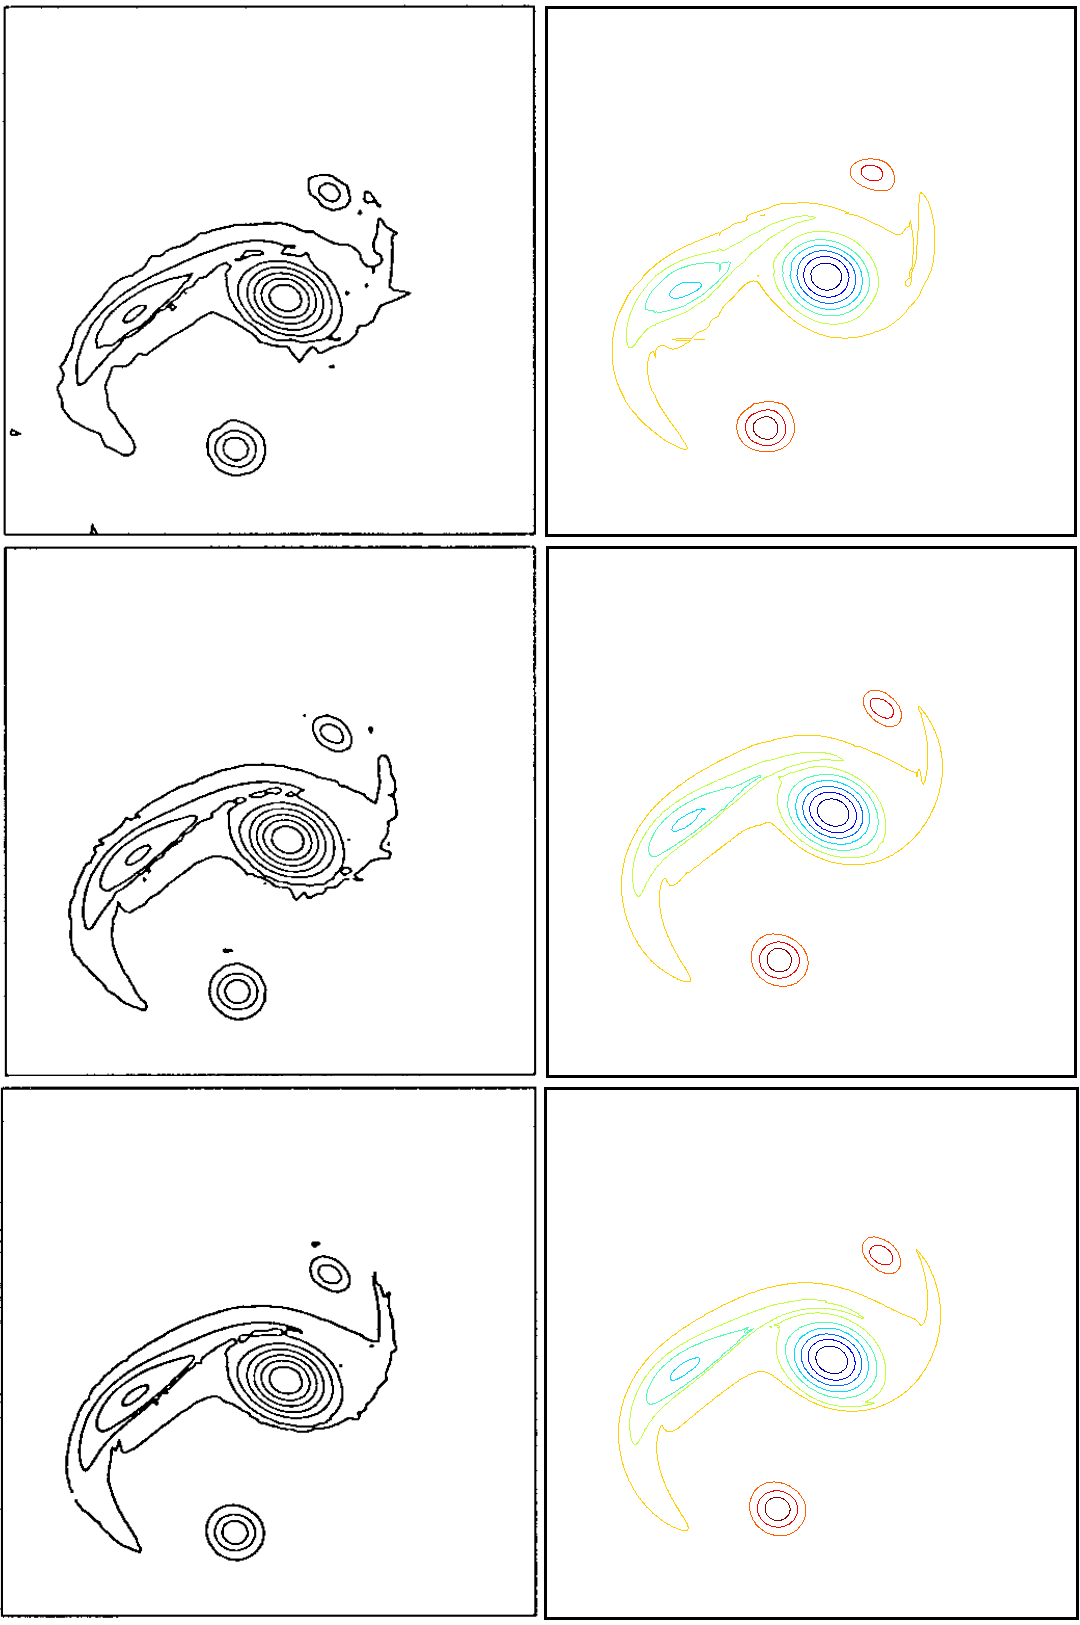
\includegraphics[width=1\textwidth]{StrainComp.PNG}
\caption{\label{fig:StrainComp}Comparison of Strain \cite{Strain1996} (left) with present method (right) t=28. Top to bottom, left to right: DOF= 6400, 12800, 25600; 3136, 7056, 63504. Contour interval for right column specified in \S\ref{SComp}. Reprinted with permission \cite{StrainLic}. }
\end{figure}

%
\subsection{Stage vs. Step-wise Velocity Evaluation}\label{SvsS}
In comparison to the Perlmann test case, Strain's test case has vortices that move and distort with respect to time. In this respect a stationary vortex lacks adequate discriminatory ability to compare stage vs. step-wise velocity evaluation. Therefore any difference is of interest with the present test case. In order to be able to make a quantitative comparison lower degree of freedom solutions are compared against a pseudo-exact solution with far more elements. The expectation is that the error in the higher degree of freedom solution with respect to an exact solution will be dwarfed by the error of the lower degree of freedom solutions.

Figure \ref{fig:StrainStageVSStep} compares a sixth order method with 24$\times$24 elements with respect to a sixth order method with 48$\times$48 elements. Both stage and stepwise solutions are presented with $\Delta t=0.32$. A large difference between the two solutions can be seen, with the step-wise evaluation having almost an order of magnitude larger error. The time-step was reduced to $\Delta t=0.02$ for the step-wise evaluation, with the solution having nearly as small an error as the stage-wise evaluation. A final test was performed with $\Delta t=0.0025$ for a step-wise evaluation and the $L^2$ error was equal to within nearly machine precision that of the stage-wise evaluation.

Additionally, the effect of the time-step for stage-wise evaluation was evaluated for a range of values; some were much smaller than $\delta t=0.32$, or larger as well (up to the limit of the CFL condition), with no discernible effect on the $L^2$ error of rate of convergence of vorticity.

\begin{figure}
\centering
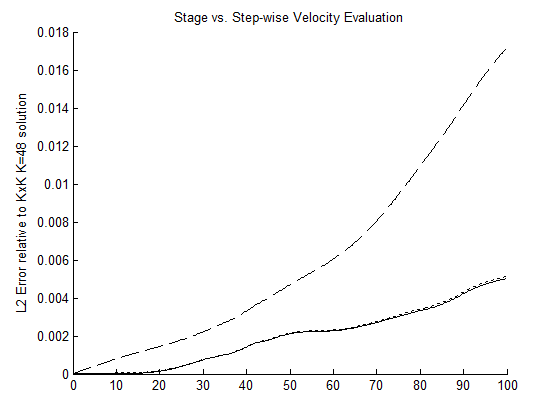
\includegraphics[width=1\textwidth]{StrainStageVSStep.PNG}
\caption{\label{fig:StrainStageVSStep}Comparison of $L^2$ vorticity error stage vs. step-wise velocity evaluation for a fourth order method with $24^2$ elements relative to a sixth order $48^2$ element solution: stage-wise $\Delta t=0.32$ (-), step-wise $\Delta t=0.32$ (- -), step-wise $\Delta t=0.02$ (..). }
\end{figure}
%
\subsection{Approximated Convergence Rates of Various Orders}\label{SConverge}
Following the same approach as \S\ref{SvsS} a solution with far more elements was used to calculate the $L^2$ error in less refined test. In this case a sixth order 60$\times$60 element solution was used as the comparative solution. A time-step of $\delta t=0.32$ was chosen to satisfy the CFL condition in all tests allowing the time-step to be kept constant across all tests.

A fourth order and sixth order method were chosen to examine the rate of convergence for the Strain test case. Solver parameters (most notably $\delta$) were chosen to minimize the $L^2$ error at t=28s. Figure \ref{fig:StrainL2} presents the $L^2$ error for the sixth order method for the element range studied, which is indicative of the approximate order of magnitude of error that was observed in this range of degrees of freedom amongst various order methods.

\begin{figure}
\centering
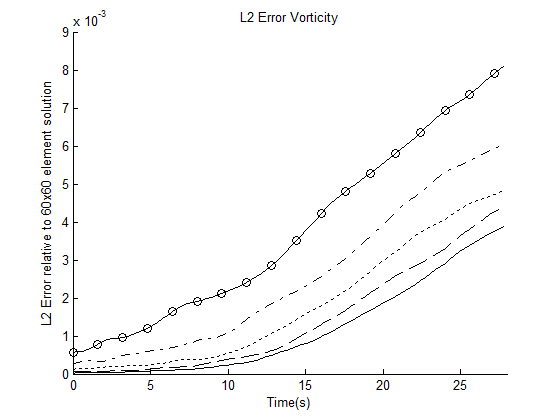
\includegraphics[width=1\textwidth]{StrainL2.PNG}
\caption{\label{fig:StrainL2}Comparison of $L^2$ vorticity error in a fourth order method, $K^2$ elements relative to a $60^2$ element solution: K= 11(-o), 14(-.), 17(..), 19(- -), 23(-). }
\end{figure}

Figure \ref{fig:Strain4vs6} compares the rate of convergence of the two methods. Although each method initially displays optimal convergence, the convergence rate decays over time until the two display approximately the same evolution. This decay of the convergence order appears similar to the behavior of too small a cutoff radius, so a further set of tests was performed for the sixth order method with a larger $\delta$. The result is plotted in Figure \ref{fig:Strain6vs6} compared against the 6th order result also in \ref{fig:Strain4vs6}. The order of convergence is far better at later times than the smaller cutoff radius test, but is limited to approximately 3rd order convergence, nowhere near optimal convergence.

\begin{figure}
\centering
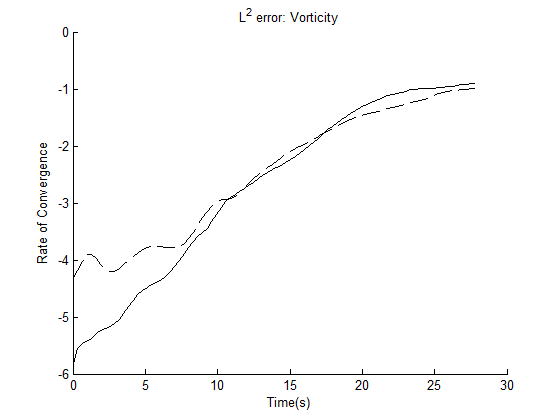
\includegraphics[width=1\textwidth]{Strain4vs6.PNG}
\caption{\label{fig:Strain4vs6}Dependency of rate of convergence on order of method, for a 4th order(- -) and 6th order(-) method. }
\end{figure}
\begin{figure}
\centering
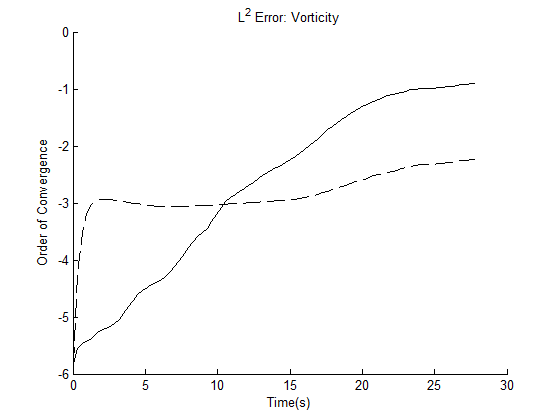
\includegraphics[width=1\textwidth]{Strain6vs6.PNG}
\caption{\label{fig:Strain6vs6}Dependency of rate of convergence on cutoff radius in sixth order method, for a $\delta/\Delta x$= 0.5(- -) and 0.25(-). }
\end{figure}
%
\subsection{Conservation of Vorticity and Linear Impulse}
In all convergence test cases vorticity was conserved to within 0.03\% and linear impulse to within 2E-5. Very little improvement in the conservation of linear impulse was seen, even as the element size decreased. On the other hand the conservation of vorticity did converge, but not at the rate of the order of the method (see Figure \ref{fig:StrainConserve}. As was seen in the Perlmann test case in \S\ref{PConserveW}, the convergence rate of invariants is somewhat dependent on the nature of the vortex system.
\begin{figure}
\centering
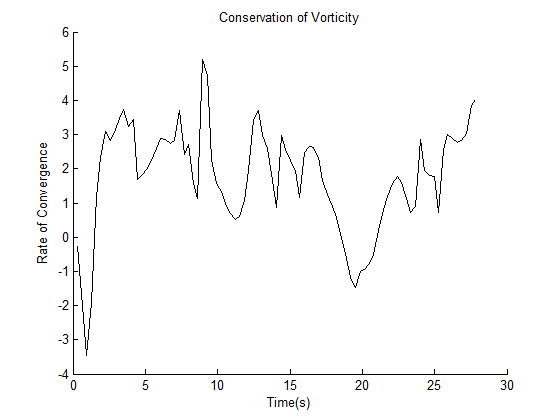
\includegraphics[width=1\textwidth]{StrainConserve.PNG}
\caption{\label{fig:StrainConserve}Rate of convergence of the conservation of vorticity for sixth order method, Strain test case. }
\end{figure}

%%
\section{Koumoutsakos: Elliptical Vortex}
%
\subsection{Comparison with Originally Published Results}\label{KoumComper}
Although an analytical solution does not exist for the given vortex system, we shall compare the solution from the present method with that obtained by Koumoutsakos \cite{Koum1997}. Identical contour intervals were used (0.25, 0.5, 1, 2, ...,20) and the solution was observed at similar times. The smoothness of the initial vorticity configuration is limited by the polynomial generating function, so a 4th order method was used with $30^2$ elements and a $\delta/\Delta x=0.4$. In order to satisfy the CFL condition a time-step of 0.0104 seconds was necessary.

Figures \ref{fig:KoumComp1}, \ref{fig:KoumComp2}, and \ref{fig:KoumComp3} compare the evolution of the solution obtained from the present method with the results of Koumoutsakos. With the exception of some numerical artifacts near regions of strong vorticity gradients, all of the plots agree very well. The comparison plots at 18 and 24 seconds display some small differences.

It is uncertain whether the third observation time is rounded in \cite{Koum1997}, as the time reported doesn't match up with the expected vortex behavior. The first 3 evolution plots shown in \cite{Koum1997} correspond to 0.5, 1.25, and 1.5 revolutions respectively; if the first half revolution were to occur in the reported 1 second, than 1.5 revolutions should take 3 seconds not the reported 4 seconds. Furthermore, the first half rotation occurred in 0.80 seconds in the solution obtained by the present method, with 1.5 rotations occurring at 2.32 seconds. All other matching times occurred within a tenth of a second of the reported time, reasonably explained by rounding.

\begin{figure}
\centering
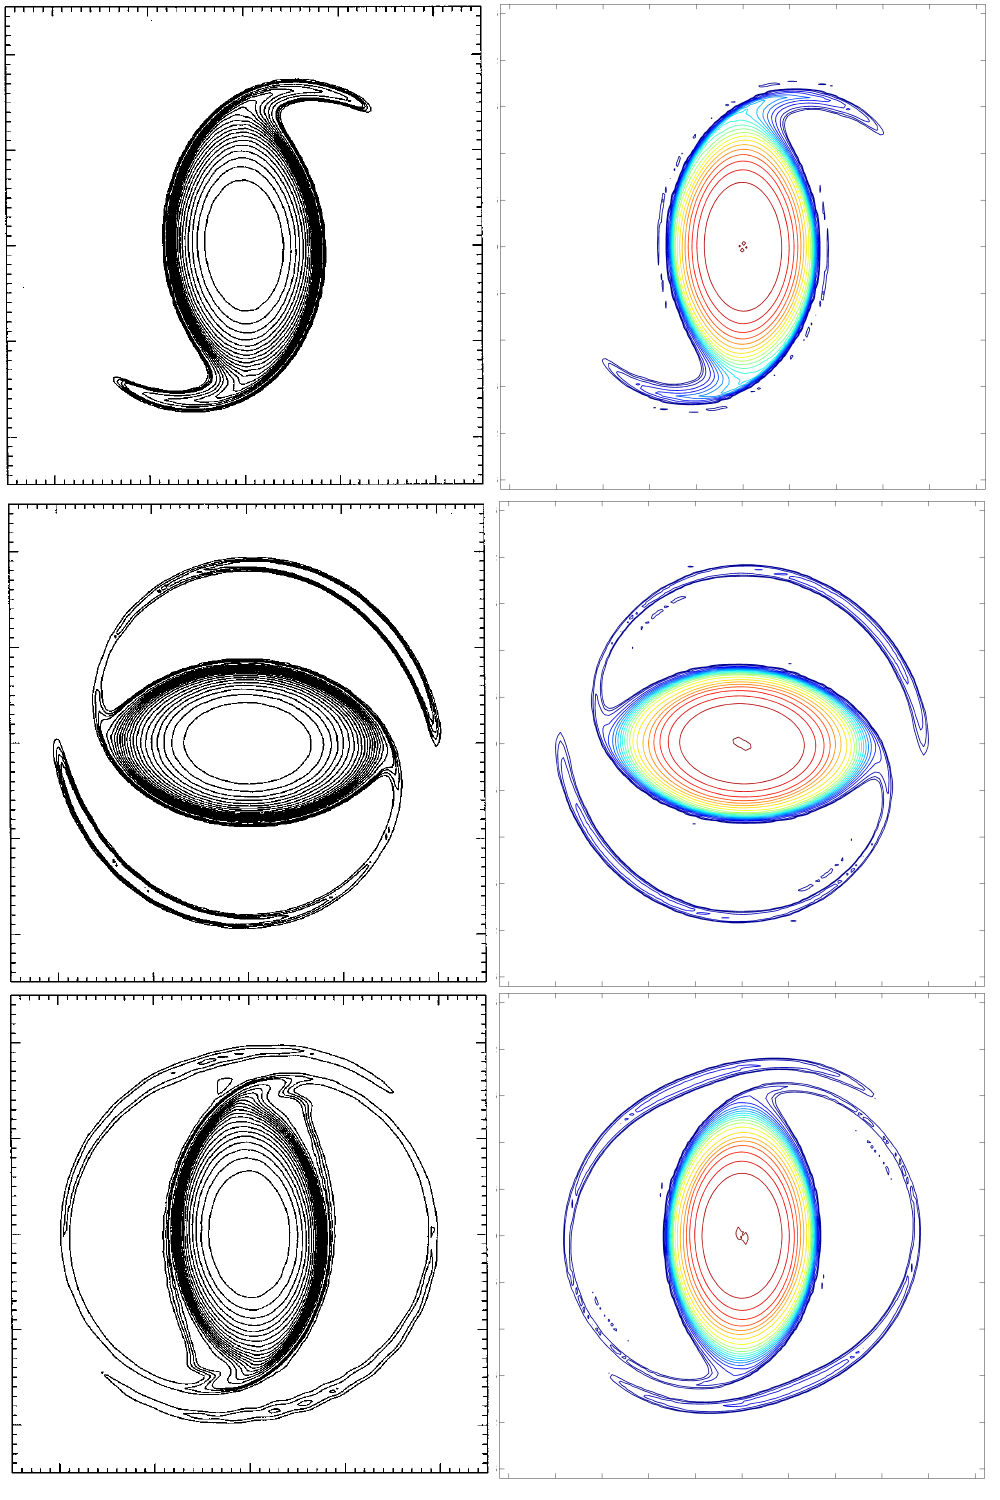
\includegraphics[width=1\textwidth]{KoumComp1.PNG}
\caption{\label{fig:KoumComp1}Comparison of vorticity, Koumoutsakos \cite{Koum1997} (left) and present method (right). From top to bottom, left to right: t=1, 2, 4; 0.80, 1.93, 2.32. Reprinted with permission \cite{KoumLic}.}
\end{figure}
\begin{figure}
\centering
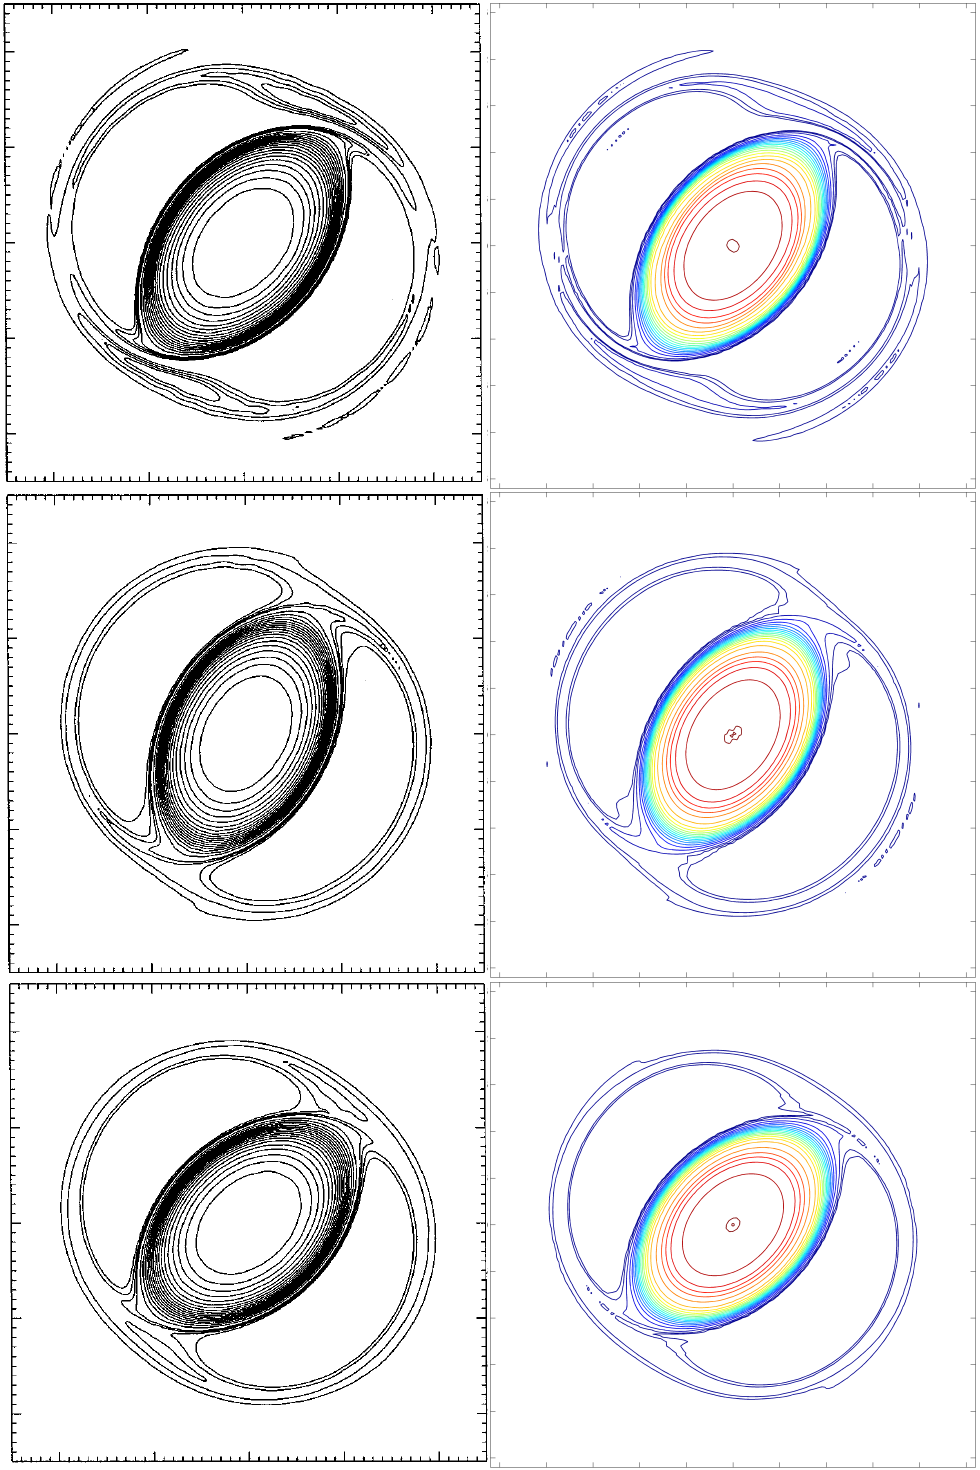
\includegraphics[width=1\textwidth]{KoumComp2.PNG}
\caption{\label{fig:KoumComp2}Comparison of vorticity, Koumoutsakos \cite{Koum1997} (left) and present method (right). From top to bottom, left to right: t=6, 12, 18; 5.94, 11.99, 17.94. Reprinted with permission \cite{KoumLic}.}
\end{figure}
\begin{figure}
\centering
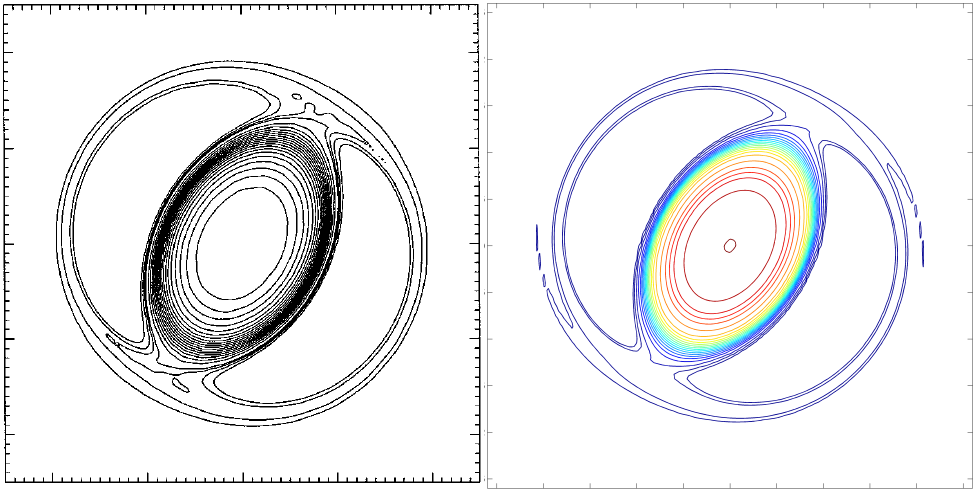
\includegraphics[width=1\textwidth]{KoumComp3.PNG}
\caption{\label{fig:KoumComp3}Comparison of vorticity, Koumoutsakos \cite{Koum1997} (left) and present method (right). From left to right: t=24; 23.98. Reprinted with permission \cite{KoumLic}.}
\end{figure}

%
\subsection{Evolution of Aspect Ratio}
One of the important features of the test case studied by Koumoutsakos in \cite{Koum1997} was it's non-axisymmetrization. The time evolution of the ellipticity was monitored by observing the change of the effective aspect ratio with respect to time. This provides an additional method of comparison between the results of the present method and  \cite{Koum1997}.

Figure \ref{fig:AspectRatio} compares the evolution of the two effective aspect ratios, the solver parameters were identical to those used in \S\ref{KoumComper}. The plots agree well, with the most pronounced difference being the amplitude of the peaks in the quasi-steady state for $t>17$ is greater than the results obtained in \cite{Koum1997}.
\begin{figure}
\centering
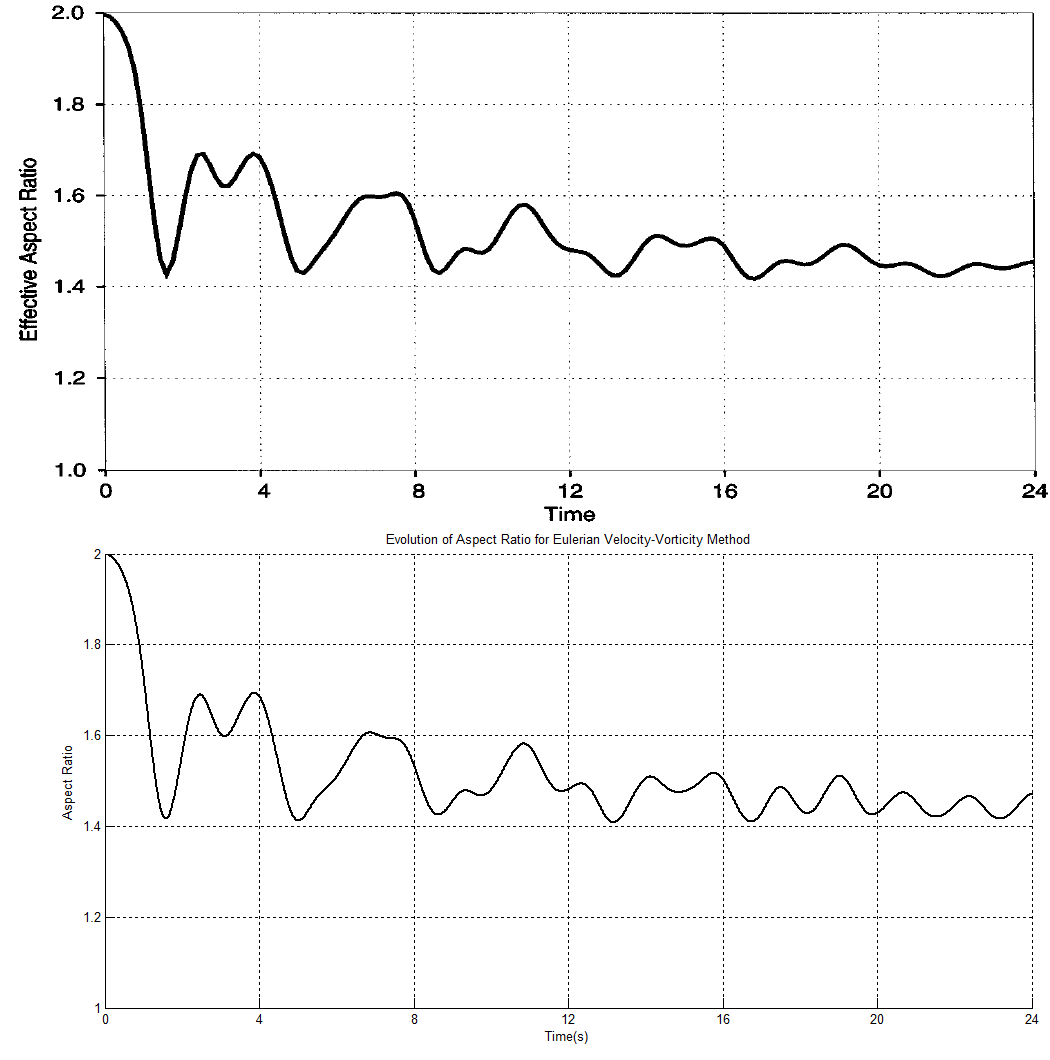
\includegraphics[width=1\textwidth]{AspectRatio.PNG}
\caption{\label{fig:AspectRatio}Comparison of effective aspect ratio, Koumoutsakos \cite{Koum1997} (top) and present method (bottom). Reprinted with permission \cite{KoumLic}.}
\end{figure}
%
\subsection{Approximated Convergence Rates of Various Orders}
We would like to follow a similar approach to that taken in \S\ref{SConverge}, however a problem presents itself. Solutions with lower element counts are insufficiently converged to provide a meaningful comparison of convergence rates. Figure \ref{fig:KoumNonConverge} compares the would-be pseudo-exact solution compared to what would be one of the test cases used in the calculation of convergence. Large spurious vortex patches are present in the 12 element solution, the arm filaments are too large, and the attachment point to the main vortex body is quite different.

Present computational constraints preclude the proper estimation of a convergence rate as the test cases would require approximately $30^2$ elements, with the validating solution likely requiring in the neighborhood of $60^2$ elements.

\begin{figure}
\centering
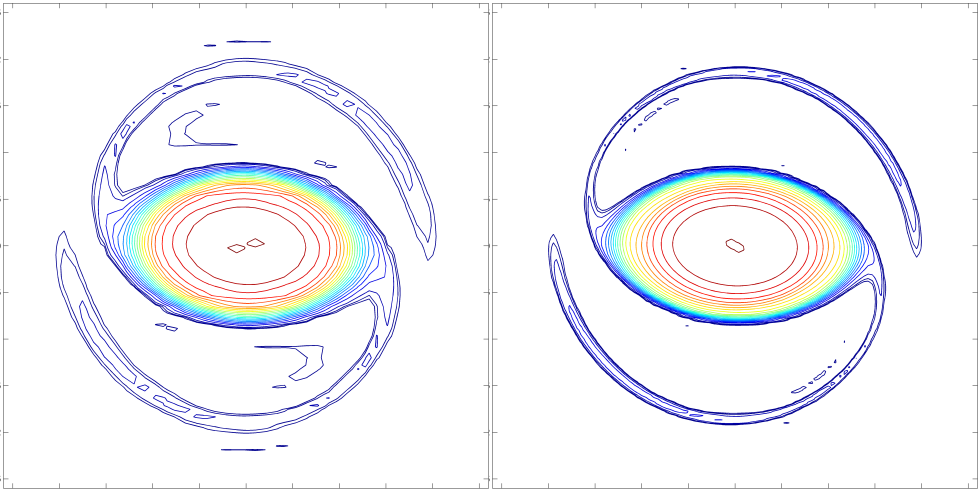
\includegraphics[width=1\textwidth]{KoumNonConverge.PNG}
\caption{\label{fig:KoumNonConverge}Comparison of solutions at t=1.93, 4th order method with $K^2$ elements: K=12 (left), 30 (right).}
\end{figure}
%
\subsection{Conservation of Vorticity}
Figure \ref{fig:KoumWConserve} plots the conservation of vorticity for the 4th method as described in \ref{KoumComper}. The cyclical nature is due to temporary production of non-physical vorticity artifacts. Additionally linear impulse was conserved within machine precision for the same solution.

\begin{figure}
\centering
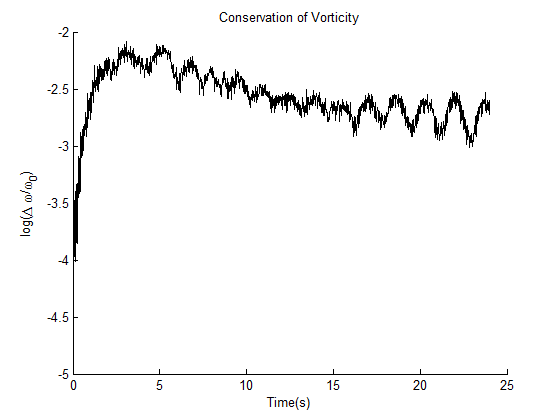
\includegraphics[width=1\textwidth]{KoumWConserve.PNG}
\caption{\label{fig:KoumWConserve}Conservation of vorticity in fourth order method, $30^2$ elements.}
\end{figure}

%------------------------------------
\chapter{Discussion}
\section{Validation}
Before the convergence rate can be examined, validation of the high-order Eulerian vorticity-velocity method should be discussed.
\subsection{Agreement where an Analytical Solution Exists}
The test case in \cite{Perlmann1985} provides an analytical solution to the initial vortex configuration. Given the choice of a spectral kernel with velocity order equal to vorticity order, stage-wise velocity evaluation, and a correctly chosen cutoff radius as determined in \S5.2.1-5.2.4 the method can robustly calculate both the evolution of vorticity and the resultant velocity field to within the limits of the discretization. 

For illustrative purposes consider the experiments done in \S5.2, the $L^2$ error in vorticity of the sixth order method with only 2401 degrees of freedom was less than 1E-6 at t=20s, vorticity was conserved within 3E-7, and linear impulse was conserved to within machine precision.
\subsection{Qualitative Agreement with Known Results}
The Strain \cite{Strain1996} and Koumoutsakos \cite{Koum1997} test cases are far more challenging than the analytical test case. Large localized vorticity gradients present challenges for the polynomial basis on a constant size grid. Qualitatively however the results presented match quite well with the published results.

The solution of the interacting vortex patches in \S5.3.1 is nearly converged with only 3136 degrees of freedom, compared to the N=25600 necessary for the result of Strain in Figure \ref{fig:StrainComp}. The $L^2$ error in vorticity for a fourth order method with $23^2$ elements in Figure \ref{fig:StrainL2} was less than 4E-3. All cases examined were able to conserve vorticity to within 0.03\% and linear impulse to within 2E-5.

The solution of the elliptical vortex in \S5.4.1 likewise agreed exceptionally well with published results. Even the fine vortex filaments that evolve from the main vortex body were properly resolved, despite the fact that the vorticity in these regions is typically less 3\% of the maximum vorticity in the domain. 

The accurate resolution of the filaments comes at the price of requiring approximately the same number of degrees of freedom as was used in \cite{Koum1997}, despite using a fourth order method in these results. Adaptive meshing or polynomial basis refinement is not employed in the current method, the strong vorticity gradients at the boundary of the main vortex body and in the arm filaments occur over so small an area that decreasing the element size doesn't result in more elements spanning these regions for the order of magnitude of degrees of freedom employed. A decrease in mesh size does however permit a larger portion of the polynomial basis in a particular element to be used to discretize these regions, resulting in a more gradual convergence in these areas.

\section{Convergence Rate}
The convergence rate for the high-order Eulerian vorticity-velocity method is dependent on not only the order of the method employed, but also on the nature of the flow solved. The convergence rate plotted in Figure \ref{fig:Porder} is very nearly optimal, with a loss of half an order in the higher order methods. The loss of this half an order can be attributed to the lack of many higher order derivatives. The optimal convergence of a discontinuous Galerkin advective method is dependent on the smoothness of the flow \cite{HestWar}. Additionally, the convergence characteristics of the approximation error of an interpolating polynomial are bounded largely by the smoothness of the function being approximated \cite{Roni}.

The semi-quantitative comparison between more and less mesh-refined solutions, such as in the Strain and Koumoutsakos cases, is one that is fairly uncommon in the published literature of Lagrangian vortex methods. Even in \cite{Strain1996} where a high-order Lagrangian method is developed, the only quantitative evaluation of rate of convergence was performed for the Perlmann test case \cite{Perlmann1985}. In this respect, examination of the order of convergence in these far more challenging test cases is a very challenging test.

The order of convergence achievable in the Strain test case did initially match the order of the underlying method as plotted in \ref{fig:Strain4vs6}, however it decayed over time to eventually a first order convergence. Interestingly the 4th order solution maintained it's convergence rate until the solution progressed to the point at which the 6th order solution had decayed to fourth order. At this point both solutions decayed at roughly the same rate. The decay of the order of convergence will be discussed in \S\ref{Decay}

\subsection{Decay of Convergence Rate}\label{Decay}
The effect of less smooth flows may partly explain why the convergence decayed in the Strain test case. The phenomenon appears similar to the behavior of the convergence rate of solutions to the Perlmann test case that had too small of a cutoff radius (see Figure \ref{fig:CutoffW}). In order to maintain a reasonably small approximation error in the velocity field the cutoff radius must be small. However if certain regions of the flow have rapidly changing non-monotonic behavior, the resulting quadrature error in the Biot-Savart integral will be larger. The result is it is not possible to choose a cutoff radius that gives both an acceptable quadrature error \textit{and} approximation error for the velocity.

Compare \ref{fig:Strain4vs6} with Figure \ref{fig:Strain6vs6}; both the 4th and 6th order methods in the former eventually decaying to a first order convergence rate. In comparison, choosing double the cutoff radius for the 6th order method in the second figure allows the sixth order method to maintain approximately a 3rd order convergence. This disparity indicates that the smaller cutoff radius is actually providing an accurate enough velocity approximation for the needs of that order method, but the quadrature error is too large and over time the method loses optimal convergence. The increased cutoff radius is able to maintain it's order of convergence because the quadrature error is small enough to not appreciably accumulate, but the additional smoothing added to the Biot-Savart kernel limits the order of accuracy of the calculated velocity and therefore the overall method.

\subsection{Generation of Non-physical Artifacts}
One other item that results from strong vorticity gradients and lack of local derivatives is the generation of non-physical vorticity artifacts in these regions. As an example consider the top right plot in Figure \ref{fig:KoumComp1}. The initial vorticity configuration (Eqn.\,\eqref{KoumEqn} is piecewise continuous at it's surface where it transitions to zero, however none of it's derivatives are continuous. As a result small non-physical oscillations in the local approximating polynomials can result. This is particularly noticeable around the periphery of the surface of the main vortex body.

The artifacts produced are only 1\% of the maximum vortex strength and are short lived, so they should have minimal effect on the overall evolution of the vortex. They do however increase the $L^2$ error of the solution. The strength and frequency of these oscillations should decrease with increased polynomial order and decreased element sizes, so solutions with more degrees of freedom should ameliorate this issue. It should be noted that this is a problem somewhat particular to an Eulerian approach, however Lagrangian vortex methods can also generate non-physical artifacts during re-meshing with higher order kernels where positivity is not guaranteed \cite{Koum1997}.

%------------------------------------
\chapter{Conclusion}
\section{Summary}
The overarching thesis goal was the development of a high-order solver capable of modeling inviscid incompressible vorticity-dominated flows in 2D. An advective solver capable of mixed order flux handling was constructed capable of high-order convergence. Additionally a high-order Biot-Savart evaluation routine using a direct summation approach was created to keep the underlying approach as efficient as possible while attempting to remove potential performance problems.

The result is a complete high-order method for velocity-vorticity inviscid flow that integrates all necessary subsystems. Both the solver and the underlying Eulerian vortex approach were validated against analytical and qualitative test cases. Finally, the $L^2$ error, vortex diagnostics, and convergence rate were measured. The method was shown capable of achieving near optimal convergence rate in smooth flows. In flows where vorticity is changing rapidly spatially the method suffers from insufficient Biot-Savart quadrature convergence. However, if an improvement were to be made to the ability of the quadrature routine to integrate the nearly singular Biot-Savart kernel it may be possible to maintain overall convergence of the method without decay.

\section{Recommendations}
\subsection{Expansion of Method Generality}
There are several additions that could be made to the high-order Eulerian velocity-vorticity method that would increase the generality of it's applicability.
\begin{itemize}
\item The extension to 3D would permit the investigation of any number of interesting phenomenon that lack 2D analogues (collision of vortex rings \cite{Wee} being a common 3D test case). The vortex stretching operator would need to be accounted for, but it's calculation is easier than for most Lagrangian methods thanks to the Eulerian grid \cite{Saffman1992}.

\item Viscosity is an important physical phenomenon currently not accounted for with the inviscid method presented. Some Lagrangian methods attempt to model viscosity by exchange of vorticity between neighboring vortex blobs during remeshing \cite{HaldReview}. By contrast rather than attempting to model this exchange, an Eulerian approach would be to use the existing grid and calculate a solution to the diffusive operator. This would enable the study of interesting phenomena like vortex merging and reconnection.

\item Impinging geometry within the domain typically creates vorticity if viscous effects are included. Additionally, even for inviscid flows boundary conditions would need to be imposed to ensure no flow through the surface. This would involve solution of the uncorrected velocity field and then correction accounting for the boundary conditions. Being able to properly simulate vorticity generation within the domain would permit the study of any number of interesting external flow problems (e.g. wind turbines, airplanes, helicopters, etc.).
\end{itemize}

\subsection{Speed or Accuracy Improvements}
Additionally several other improvements could be made to increase the speed or accuracy of the overall method:
\begin{itemize}
\item The largest improvement to accuracy would be the implementation of an integration procedure for the singular Biot-Savart integral for self-influence and nearly singular integral for neighboring elements. This may also lead to relative speed improvements as well; the overall runtime would not be reduced, but the runtime required for a particular level of accuracy should be reduced. This would reduce or outright remove the need to de-singularize the Biot-Savart kernel, resulting in improved convergence of the overall method by reducing the balancing effect necessary in the selection of the cutoff radius.
\item The implementation of a flux limiter would permit the preservation of the sparsity of vorticity and prevent vorticity noise from spreading to what should be otherwise empty elements. Currently advective calculations are only a small fraction of the computational budget, but if the cost of velocity evaluations were to be reduced advective calculations could necessitate a speedup in evaluation.
\item Implict time-stepping would be very useful, especially for high-order solutions with many elements where solution stiffness dictates a time-step far smaller than may be of interest. Fast reduced velocity order or step-wise velocity evaluation solutions could be potentially used a pre-conditioner for the full order method.
\item For practical scalability to application on large or complex problems the underlying code base should attempt to be parallelized for computation on clusters.
\item Application of a Fast Multipole Method \cite{GreengardRokhlin1987} could drastically reduce the cost of velocity evaluations, although the spectral kernel could not be used for the de-singularized Biot-Savart integral due to the non-compact support. Instead, a kernel with compact support would need to be used.
\end{itemize}

\subsection{Major Structural Changes}
Finally, major structural changes to the underlying method could present new avenues of approach to obtaining solutions:
\begin{itemize}
\item Rather than taking the approach of Lagrangian methods and calculating the velocity field via the Biot-Savart integral, one could instead solve a Poisson problem for the velocity due to a vorticity configuration. The use of the Eulerian grid would simplify this and the non-physical singularities present in the Biot-Savart kernel could be avoided entirely, possibly eliminating the vorticity order decay observed in the Strain test case.
\item Alternatively, one could attempt non-standard quadrature methods to more accurately integrate the nearly singular de-singularized or truly singular Biot-Savart kernel. This would permit a smaller cutoff radius (or remove the need for de-singularization entirely) and reduce the approximation error in the velocity field.
\end{itemize}

%------------------------------------
\begin{thebibliography}{8}
%Overview
\bibitem{Lugt1983}
H. J. Lugt, Vortex Flow in Nature and Technology, Krieger Publishing Company, Malabar, FL, USA, 1983.
\bibitem{Saffman1992}
P. G. Saffman, Vortex Dynamics, Cambridge Univ. Press, Cambridge, UK, 1992.
\bibitem{Speziale1987}
C. G. Speziale, On the advantages of the vorticity-velocity formulation of the equations of fluid dynamics, J. Comput. Phys. 73 (1987) 476-480.
%Point methods
\bibitem{Point1}
L. Rosenhead, The formation of vorticies from a surface of discontinuity, Proc. Roy. Soc. London Ser. A 134 (1931) 170-192.
\bibitem{Point2}
G. Birkhoff, J. Fisher, Do vortex sheets roll up?, Rend. Circ. Math. Palermo, Ser. 2 8 (1959) 77-90.
\bibitem{Point3}
F. H. Abernathy, R. E. Kronauer, The formation of vortex streets, J.Fluid Mech. 13 (1962) 1-20.
\bibitem{Point4}
A. J. Chorin, P. S. Bernard, Discretization of a vortex sheet, with an example of roll-up, J. Comput. Phys. 13 (3) (1973) 423-429.
\bibitem{Point5}
K. Kuwahara, H. Takami, Numerical studies of two-dimensional vortex motion by a system of point vortices, J. Physical Society of Japan 34 (1) (1973) 247-253.
\bibitem{Point6}
R. G. Zalosh, Discretized simulation of vortex sheet evolution with buoyancy and surface tension effects, AIAA Journal 14 (11) (1976) 1517-1523.
%Line methods
\bibitem{Line1}
G. K. Batchelor, An Introduction to Fluid Dynamics, Cambridge University Press, 1967, 1973.
\bibitem{Line2}
W. T. Ashurst, E. Meiburg, Three-dimensional shear layers via vortex dynamics, J. Fluid Mech. 189 (1988) 87-116.
\bibitem{Line3}
J. E. Martin, E. Meiburg, Numerical investigation of three-dimensional evolving jets subject to axisymmetric and azimuthal perturbation, J. Fluid Mech. 230 (1991) 271-318.
\bibitem{Line4}
A. Leonard, Numerical simulation of interacting, three-dimensional vortex filaments, in: Proceedings of the IV Intl. Conference on Numerical Methods of Fluid Dynamics, no. 35 in Lecture Notes in Physics, Springer-Verlag, 1975, pp. 245-250.
%Sheet methods
\bibitem{Sheet1}
M. E. Agishtein, A. A. Migdal, Dynamics of vortex surfaces in three dimensions: Theory and simulations, Physica D 40 (1989) 91-118.
\bibitem{Sheet2}
O. M. Knio, A. F. Ghoniem, Three-dimensional vortex simulation of rollup and entrainment in a shear layer, J. Comput. Phys. 97 (1991) 172-223.
\bibitem{Sheet3}
O. M. Knio, A. F. Ghoniem, Vortex simulation of a three-dimensional reacting shear layer with in finite-rate kinetics, AIAA J. 30 (1) (1992) 105-116.
%Volume methods
\bibitem{Volumes1}
G. Russo, J. A. Strain, Fast triangulated vortex methods for the 2D Euler equations, J. Comput. Phys. 111 (1994) 291-323.
\bibitem{Volumes2}
M. Carley, A triangulated vortex method for the axisymmetric Euler equations, J. Comput. Phys. 180 (2002) 616-641.
\bibitem{Volumes3}
S. A. Huyer, J. R. Grant, Solution of two-dimensional vorticity equation on a Lagrangian mesh, AIAA Journal 38 (5) (2000) 774-783.
%Misc methods
\bibitem{MiscMeth1}
Williamson, David L. Integration of the barotropic vorticity equation on a spherical geodesic grid. Tellus 20, no. 4 (1968): 642-653.
\bibitem{MiscMeth2}
Russell, David, and Z. Jane Wang. A Cartesian grid method for modeling multiple moving objects in 2D incompressible viscous flow. Journal of Computational Physics 191, no. 1 (2003): 177-205.
\bibitem{MiscMeth3}
Calhoun, Donna. A Cartesian grid method for solving the two-dimensional streamfunction-vorticity equations in irregular regions. Journal of computational physics 176, no. 2 (2002): 231-275.
\bibitem{MiscMeth4}
Suh, J-C. The evaluation of the Biot–Savart integral. Journal of engineering mathematics 37, no. 4 (2000): 375-395.
%Remeshing problems
\bibitem{Remesh2}
J. T. Beale, On the accuracy of vortex methods at large times, in: IMA Workshop on Computational Fluid Dynamics and Reacting Gas Flows, Springer-Verlag, 1988, p. 19.
\bibitem{Remesh3}
J. S. Marshall, J. R. Grant, Penetration of a blade into a vortex core: vorticity response and unsteady blade forces, J. Fluid Mech. 306 (1996) 83-109.
\bibitem{Remesh4}
H. O. Nordmark, Rezoning for higher order vortex methods, J. Comput. Phys. 97 (1991) 366-397.
\bibitem{Remesh5}
H. N. Najm, R. B. Milne, K. D. Devine, S. N. Kempa, A coupled Lagrangian-Eulerian scheme for reacting flow modeling, ESAIM Proc. 7 (1999) 304-313.
%Convergence
\bibitem{Convg2D}
O. H. Hald, V. D. Prete, Convergence of vortex methods for Euler's equations, Math. Comput. 32 (1978) 791-809.
\bibitem{Convg3D}
J. T. Beale, A convergent 3-D vortex method with grid-free stretching, Math. Comput. 46 (174) (1986) 401-424.
%Brown
\bibitem{Brown2000}
 R.E. Brown. Rotor Wake Modeling for Flight Dynamic Simulation of Helicopters. AIAA Journal, 2000. Vol. 38(No. 1): p. 57-63.
\bibitem{Brown2004}
A.J. Line, R.E. Brown. Efficient High-Resolution Wake Modelling using the Vorticity Transport Equation. in 60th Annual Forum of the American Helicopter Society. 2004. Baltimore, MD.
%DG
\bibitem{ReedHill}
W.H Reed and T.R. Hill. Triangular mesh methods for the neutron transport equation. 1973.
\bibitem{Lesaint}
Lesaint, P., and Pierre-Arnaud Raviart. On a finite element method for solving the neutron transport equation. Mathematical aspects of finite elements in partial differential equations 33 (1974): 89-123.
\bibitem{Persson2013}
P.O. Persson. A Sparse and High-Order Accurate Line-Based Discontinuous Galerkin Method for Unstructured Meshes. J. Comp. Phys., Vol. 233, pp. 414-429, Jan 2013.
\bibitem{HestWar}
Hesthaven, Jan S., and Tim Warburton. Nodal discontinuous Galerkin methods: algorithms, analysis, and applications. Vol. 54. Springer Science \& Business Media, 2007.
\bibitem{RKDG}
Cockburn, Bernardo, and Chi-Wang Shu. TVB Runge-Kutta local projection discontinuous Galerkin finite element method for conservation laws. II. General framework. Mathematics of Computation 52.186 (1989): 411-435.
%Important vortex papers
\bibitem{HaldReview}
Hald, Ole H. Convergence of vortex methods. Vortex methods and vortex motion. Vol. 1. 1991.
\bibitem{Hald3}
Hald, Ole H. Convergence of vortex methods for Euler's equations, III. SIAM journal on numerical analysis 24.3 (1987): 538-582.
\bibitem{WL}
Winckelmans, G. S., and A. Leonard. Contributions to vortex particle methods for the computation of three-dimensional incompressible unsteady flows. Journal of Computational Physics 109.2 (1993): 247-273.
\bibitem{BealeMajda}
Beale, J. Thomas, and Andrew Majda. High order accurate vortex methods with explicit velocity kernels. Journal of Computational Physics 58.2 (1985): 188-208.
\bibitem{Strain1997}
J. Strain. Fast adaptive 2D vortex methods. Journal of computational physics 132.1 (1997): 108-122.
\bibitem{LindsayKrasny2001}
K. Lindsay, and R. Krasny. A particle method and adaptive treecode for vortex sheet motion in three-dimensional flow. Journal of Computational Physics 172.2 (2001): 879-907.
\bibitem{Rosenhead1930}
L. Rosenhead. The spread of vorticity in the wake behind a cylinder, Proc. Roy. Soc. London Ser. A 127, 590 (1930).
\bibitem{Moore1972}
D. W. Moore. Finite amplitude waves on aircraft trailing vortices, Aero. Quart. 23, 307 (1972).
\bibitem{MoussaCarley2008}
Moussa, C., Carley, M. J. (2008). A Lagrangian vortex method for unbounded flows. International journal for numerical methods in fluids, 58(2), 161-181.
\bibitem{SteinhoffUnderhill1994}
J. Steinhoff, D. Underhill, Modification of the Euler equations for ``vorticity confinement'': Application to the computation of interacting vortex rings, Phys. Fluids 6 (8) (1994) 2738-2743.
%Test cases
\bibitem{Perlmann1985}
M. Perlman. On the accuracy of vortex methods, J. Comput. Phys. 59 (1985) 200–223.
\bibitem{Strain1996}
J. Strain. 2D vortex methods and singular quadrature rules. Journal of Computational Physics 124.1 (1996): 131-145.
\bibitem{Koum1997}
P. Koumoutsakos. Inviscid axisymmetrization of an elliptical vortex, J. Comput. Phys. 138 (1997) 821–857.
\bibitem{KoumLeonard1995}
Koumoutsakos, P., Leonard, A. (1995). High-resolution simulations of the flow around an impulsively started cylinder using vortex methods. Journal of Fluid Mechanics, 296, 1-38.
\bibitem{Southerland1991}
K. B. Southerland, J. R. P. III, W. J. A. Dahm, K. A. Buch. An experimental study of the molecular mixing process in an axisymmetric laminar vortex ring, Phys. Fluids A 3 (5) (1991) 1385–1392.
%Fast velocity eval
\bibitem{SchumannSweet1976}
Schumann, U., Sweet, R. A. (1976). A direct method for the solution of Poisson's equation with Neumann boundary conditions on a staggered grid of arbitrary size. Journal of Computational Physics, 20(2), 171-182.
\bibitem{BarnesHut1986}
Barnes, J.,  Hut, P. (1986). A hierarchical O (N log N) force-calculation algorithm.
\bibitem{GreengardRokhlin1987}
Greengard, L.,  Rokhlin, V. (1987). A fast algorithm for particle simulations. Journal of computational physics, 73(2), 325-348.
%General ortho bases
\bibitem{Gasca2000}
Gasca, Mariano, Thomas Sauer. Polynomial interpolation in several variables. Advances in Computational Mathematics 12.4 (2000): 377-410.
\bibitem{Xu2012}
Xu, Yuan. Minimal Cubature rules and polynomial interpolation in two variables. Journal of Approximation Theory 164.1 (2012): 6-30.
\bibitem{Gautschi2013}
Gautschi, Walter. Neutralizing nearby singularities in numerical quadrature. Numerical Algorithms 64.3 (2013): 417-425.
%LSERK
\bibitem{Reid}
Atcheson, Thomas. Explicit Discontinuous Galerkin Methods for Linear Hyperbolic Problems. Diss. Masters Thesis, Rice University. http://hdl. handle. net/1911/75120, 2013.
\bibitem{Toulorge}
Toulorge, Thomas, and Wim Desmet. Optimal Runge–Kutta schemes for discontinuous Galerkin space discretizations applied to wave propagation problems. Journal of Computational Physics 231.4 (2012): 2067-2091.
\bibitem{Niegemann}
Niegemann, Jens, Richard Diehl, and Kurt Busch. Efficient low-storage Runge–Kutta schemes with optimized stability regions. Journal of Computational Physics 231.2 (2012): 364-372.
\bibitem{Carpenter}
Carpenter, Mark H., and Christopher A. Kennedy. Fourth-order 2N-storage Runge-Kutta schemes. (1994).
%Misc
\bibitem{Roni}
Quarteroni, Alfio, and Alberto Valli. Numerical approximation of partial differential equations. Vol. 23. Springer Science \& Business Media, 2008.
\bibitem{Allen}
Allen, Myron B., and Eli L. Isaacson. Numerical analysis for applied science. Vol. 35. John Wiley \& sons, 2011.
\bibitem{Gustaf}
Gustafsson, Bertil. Fundamentals of Scientific Computing. Vol. 8. Springer Science \& Business Media, 2011.
\bibitem{ButcherSurvey}
Butcher, John C. Numerical methods for ordinary differential equations in the 20th century. Journal of Computational and Applied Mathematics 125.1 (2000): 1-29.
\bibitem{Wee}
Wee, Daehyun, et al. Convergence characteristics and computational cost of two algebraic kernels in vortex methods with a tree-code algorithm. SIAM Journal on Scientific Computing 31.4 (2009): 2510-2527.
%Licenses
\bibitem{KoumLic}
Reprinted from  Journal of Computational Physics, 138, P. Koumoutsakos, Inviscid axisymmetrization of an elliptical vortex, 821–857, Copyright (1997), with permission from Elsevier.
\bibitem{StrainLic}
Reprinted from Journal of Computational Physics, 124.1, J. Strain, 2D vortex methods and singular quadrature rules, 131-145, Copyright (1996), with permission from Elsevier.
\end{thebibliography}

\cleardoublepage
\appendix
\addcontentsline{toc}{chapter}{Appendices}
%
\chapter{Notable Code and Algorithms}\label{Algs}
\section{Modified Two-part quadrature}
\singlespacing
\begin{lstlisting}[language=Matlab]
function [W,Ll,Lr] = StiffnessQuadModWeights(Qx,Qx2)
%Returns the M,N,N matrix of modified quadrature weights
%associated with the N quadrature nodes Qx and M nodes
%Qx2 for each weighting basis m<=M. Qx should be the 
%conserved quantity and Qx2 the flux velocity. This 
%quadrature is used to produce a stiffness matrix that
%is the integral of the product of two interpolations times 
%the spatial deriavitve of the weighting function. This is 
%distinct from the integral of the interpolation of the product 
%of two functions times the derivative of the weighting 
%function, and more accurate. It also permits the use of
%mixed quadrature, i.e. different order quadrature for 
%each interpolation as well as differnet nodes (GL mixed 
%with LGL for instance).
N=length(Qx);
M=length(Qx2);
%All points except the basis point for each basis
nn=elim(Qx(1:N)',Qx(1:N)',[1 3 2]);
%Associated Lagrange basis function
Lag1= @(x,nv) prod(bsxfun(@rdivide,bsxfun(@minus,x,nn(nv,:,:)),...
	bsxfun(@minus,Qx(nv),nn(nv,:,:))),3);
nn2=elim(Qx2(1:M)',Qx2(1:M)',[1 3 2]);
Lag2= @(x,nv) prod(bsxfun(@rdivide,bsxfun(@minus,x,nn2(nv,:,:)),...
	bsxfun(@minus,Qx2(nv),nn2(nv,:,:))),3);
dLag1= @(x,nv) Lag1(x,nv).*sum(1./bsxfun(@minus,x,nn(nv,:,:)),3);

W=zeros(M,N,1,N);
for j=1:N
    for i=1:M
        for n=1:N
            trip=@(x) Lag1(x,j).*Lag2(x,i).*dLag1(x,n);
            W(i,j,1,n)=integral(...
		trip,-1,1,'RelTol',1e-14,'AbsTol',1e-15);
        end
    end
end

Ll=Lag1(-1,1:N);
Lr=Lag1(1,1:N);
end
\end{lstlisting}
\doublespacing

\section{Modified Quadrature Convergence Verification}
The following script allows investigation of the convergence properties of the modified quadrature routine used. The quadrature routine can be compared to Matlab's $integral$ routine which is computed to within machine precision for validation purposes.

\singlespacing
\begin{lstlisting}[language=Matlab]
%Matrix Q contains the result of the convergence tests
P=8;
[Qx,Qw]= GLquad(P);
pp=elim(Qx(1:P)',Qx(1:P)',[1 3 2]);
Lag3= @(x,nv) prod(bsxfun(@rdivide,bsxfun(@minus,x,pp(...
	nv,:,:)),bsxfun(@minus,Qx(nv),pp(nv,:,:))),3);

R=10;
[Qx2,Qw2]= GLquad(R);
rr=elim(Qx2(1:R)',Qx2(1:R)',[1 3 2]);
Lag4= @(x,nv) prod(bsxfun(@rdivide,bsxfun(@minus,x,rr(...
	nv,:,:)),bsxfun(@minus,Qx2(nv),rr(nv,:,:))),3);

s = @(x) sin(pi*x);
    c2 = 40/100;
    b=-.2;
g = @(x) exp(-(x-b).^2/(2*c2));
s_g=@(x) s(x).*g(x);

for N=3:15
    [nd,w] = GLquad(N);
    M=N+1;
    [nd2,w2] = GLquad(M);
    
    %Fully vectorized for both x and nv
    nn=elim(nd(1:N)',nd(1:N)',[1 3 2]);
    Lag= @(x,nv) prod(bsxfun(@rdivide,bsxfun(@minus,x,nn(...
	nv,:,:)),bsxfun(@minus,nd(nv),nn(nv,:,:))),3);
    nn2=elim(nd2(1:M)',nd2(1:M)',[1 3 2]);
    Lag2= @(x,nv) prod(bsxfun(@rdivide,bsxfun(@minus,x,nn2(...
	nv,:,:)),bsxfun(@minus,nd2(nv),nn2(nv,:,:))),3);
    dLag= @(x,nv) Lag(x,nv).*sum(1./bsxfun(...
	@minus,x,nn(nv,:,:)),3);
    
    interp_s=@(x) s(nd')*Lag(x,1:N);
    interp_g=@(x) g(nd2')*Lag2(x,1:M);
    interp_s_g=@(x) s_g(nd2')*Lag2(x,1:M);
    interp_sg=@(x) interp_s(x).*interp_g(x);
    
    n=floor(N/2);
    exact=@(x) s_g(x).*dLag(x-eps(x),n);
    stiff_s_g=@(x) interp_s_g(x).*dLag(x-eps(x),n);
    stiff_sg=@(x) interp_s(x).*interp_g(x).*dLag(x-eps(x),n);
    
    Q(N,3)=integral(exact,-1,1,'RelTol',1e-14,'AbsTol',1e-16);
    Q(N,4)=integral(stiff_s_g,-1,1,'RelTol',1e-14,'AbsTol',1e-16);
    Q(N,5)=integral(stiff_sg,-1,1,'RelTol',1e-14,'AbsTol',1e-16);
    
    Q(N,6)=stiff_s_g(Qx')*Qw';
    Q(N,7)=stiff_sg(Qx')*Qw';
        
    for i=1:P
        duo=@(x) Lag3(x,i).*dLag(x,n);
        W(i)=integral(duo,-1,1,'RelTol',1e-14,'AbsTol',1e-15);
    end
    Q(N,8)=interp_s_g(Qx')*W';
    
    for i=1:P
        for j=1:R
                trip=@(x) Lag3(x,i).*Lag4(x,j).*dLag(x,n);
                W2(i,j)=integral(trip,-1,1,'RelTol',1e-14,'AbsTol',1e-15);
        end
    end
    Q(N,9)=interp_s(Qx')*(W2*interp_g(Qx2')');
    
    Q(N,15)=(N-1)+(M-1);
    Q(N,16)=N;
end
Q(:,1)=Q(:,3)-Q(:,4);
Q(:,2)=Q(:,3)-Q(:,5);

Q(:,11)=Q(:,4)-Q(:,6);
Q(:,12)=Q(:,4)-Q(:,8);
Q(:,13)=Q(:,5)-Q(:,9);
Q(:,14)=Q(:,3)-Q(:,9);
\end{lstlisting}
\doublespacing

\section{Binary Singleton Expansion Matrix-Vector Products}
Matlab does not permit application of the binary singleton expansion to matrix-vector and matrix-matrix products. Although it does permit application of elementwise multiplication via $bsxfun()$, it will return an error if the binary operator $@mtimes$ is used. One could instead perform the matrix-vector products slice by slice in $for()$ loops, but this is slow and unnatural mathematically. An external library is used to extend this ability to suit the purpose: $mtimesx()$. This permits very compact and readable code. In this application it also resulted in a 20x speedup in the advection portion of the code.

An example application of this can be seen in the code below. Here the x-line stiffness value is calculated for \textit{all} x-lines in an element for \textit{all} elements simultaneously. It does this by calculating the product of the the x-line velocities by the modified quadrature matrix by the vorticity (ordered appropriately in a x-line major format). The matrices are 3, 4, and 3 dimensional respectively; each has a singelton dimension that is expanded via the $mtimesx()$ routine. The result returned is the nodal stiffness value calculated for all nodes in all elements.

\singlespacing
\begin{lstlisting}[language=Matlab]
%Example non-standard bsx for matrix-vector products
Stiff_x= mtimesx(v_xE,mtimesx(QwSM,wx));
\end{lstlisting}
\doublespacing

\section{Lagrange Bases}
To properly compare quadrature errors, one requires the analytical form of the Lagrange bases and their derivatives. These are tedious to generate by hand. The following snippet generates a fully vectorized set of anonymous functions for the Lagrange bases and their derivatives for an arbitrary $N$ order set. These can be multiplied by the value of the function at the interpolation points to give the interpolating function. This can then be used in Matlab routines such as $integral()$ to calculate exact within machine precision values to validate against.

\singlespacing
\begin{lstlisting}[language=Matlab]
%Generate Gauss-Legendre quadrature points for Nth order
[nd,w] = GLquad(N);
%Fully vectorized for both x and nv
nn=elim(nd(1:N)',nd(1:N)',[1 3 2]);
%Lagrange anon function interpolates for any x
Lag= @(x,nv) prod(bsxfun(@rdivide,bsxfun(@minus,x,nn(...
	nv,:,:)),bsxfun(@minus,nd(nv),nn(nv,:,:))),3);
%Derivative of Lagrange anon function
dLag= @(x,nv) Lag(x,nv).*sum(1./bsxfun(...
	@minus,x,nn(nv,:,:)),3);
\end{lstlisting}
\doublespacing

\section{Velocity Evaluation}
Velocity evaluation in the standard implementation occurs stage-wise. New domain velocities are calculated due to the new stage's state. The most expensive operations that occur are the indexing and manipulation of the kernel values for each node.

\singlespacing
\begin{lstlisting}[language=Matlab]
v_xB(:)=0; v_yB(:)=0; v_xBF(:)=0; v_yBF(:)=0; v_xE(:)=0;
%Reshaped to col-wise element chunks
w_elem=reshape(permute(reshape(wy,Np,K(2),Np,K(1)),...
	[1 3 2 4]),1,Np^2,K(2)*K(1));
%Sum of vorticity in each elem
w_tot=abs(permute(mtimesx(w_elem,QwPre'),[3 1 2]));
mask=find(w_tot>w_thresh); %Find "important" elements
%Pre-multiply by quad weights for speed
w_elemPre=bsxfun(@times,QwPre,w_elem(:,:,mask));

v_xI= reshape(mtimesx(w_elemPre, kernel_x),1,Mp-2,Np*(...
	2*NearRange+1)^2,[]);
v_yI= reshape(mtimesx(w_elemPre, kernel_y),1,Mp-2,Np*(...
	2*NearRange+1)^2,[]);
for it=1:length(mask)
    w_source=w_elemPre(:,:,it);
    Src= mask(it);
    NsxS=Nsx(1:numS(Src),Src);
    NsyS=Nsy(1:numS(Src),Src);
    %Form specific source kernel by transforming the 
    %generalized source kernel to the specific source loc
    kernel_xB= gkernel_xB(:, [1:Np*K(2)] +Np*(K(2)-...
    Enumy(Src)), [1:K(1)+1] +(K(1)-Enumx(Src)) );
    kernel_yB= gkernel_yB(:, [1:Np*K(1)] +Np*(K(1)-...
    Enumx(Src)), [1:K(2)+1] +(K(2)-Enumy(Src)) );
    %Calculate boundary velocities
    v_xBt= permute(mtimesx(w_source,kernel_xB),[2 3 1]);
    v_xB= v_xB + v_xBt;
    v_yBt= permute(mtimesx(w_source,kernel_yB),[3 2 1]);
    v_yB= v_yB + v_yBt;
    %Form far field boundary velocities due to source,
    %add to existing far field velocities. Be sure to 
    %leave out near-field boundary velocities as these
    %will be included in the whole element evals
    v_xBFt= [v_xBt(EBl),v_xBt(EBr)]; v_xBFt(1,:,NsxS)=0;
    v_xBF= v_xBF + v_xBFt;
    v_yBFt= [v_yBt(EBb),v_yBt(EBt)]; v_yBFt(1,:,NsyS)=0;
    v_yBF= v_yBF + v_yBFt;

    %Assemble elementwise velocities for elements
    %nearby the source
    v_xE(1,:,NsxS)= v_xE(1,:,NsxS)+ [v_xBt(EBl(NsxS)),...
	 v_xI(1,:,Lsx(1:numS(Src),Src),it) ,v_xBt(EBr(NsxS))];
    v_yE(1,:,NsyS)= v_yE(1,:,NsyS)+ [v_yBt(EBb(NsyS)),...
	 v_yI(1,:,Lsy(1:numS(Src),Src),it) ,v_yBt(EBt(NsyS))];
end

\end{lstlisting}
\doublespacing

\section{Semi-discrete System Construction}
The semi-discrete system is constructed from the surface fluxes and the stiffness evaluation. The combination of the two uniquely determine the time-evolution of the system at the current time step.

\singlespacing
\begin{lstlisting}[language=Matlab]
<for each time step>
%---Advection---------------
w_lx= mtimesx(Ll',wx);      %Left interpolated vorticity
w_rx= mtimesx(Lr',wx);      %Right interpolated vorticity
w_bx= mtimesx(Ll',wy);      %Bottom interpolated vorticity
w_tx= mtimesx(Lr',wy);      %Top interpolated vorticity

%Boundary fluxes
if BCtype== 'NoInflow'
    v_xBC= v_xB; v_xBC(:,1)= min(v_xBC(:,1),0);
    v_xBC(:,end)= max(v_xBC(:,end),0);
    v_yBC= v_yB; v_yBC(1,:)= min(v_yBC(1,:),0);
    v_yBC(end,:)= max(v_yBC(end,:),0);
end
fl= abs( v_xBC(EBl) ).*( w_rx(x_km1).*(sign(v_xB(EBl))+alpha)...
	 + w_lx.*(sign(v_xB(EBl))-alpha) );
fr= abs( v_xBC(EBr) ).*( w_rx.*(sign(v_xB(EBr))+alpha)...
	 + w_lx(x_kp1).*(sign(v_xB(EBr))-alpha) );
fb= abs( v_yBC(EBb) ).*( w_tx(y_km1).*(sign(v_yB(EBb))+alpha)...
	 + w_bx.*(sign(v_yB(EBb))-alpha) );
ft= abs( v_yBC(EBt) ).*( w_tx.*(sign(v_yB(EBt))+alpha)...
	 + w_bx(y_kp1).*(sign(v_yB(EBt))-alpha) );

%Nodal total surface flux
SurfFlux_x=bsxfun(@times,fr,LrM)-bsxfun(@times,fl,LlM);
SurfFlux_y=bsxfun(@times,ft,LrM)-bsxfun(@times,fb,LlM);
%Nodal stiffness eval
Stiff_x= mtimesx(v_xBF,mtimesx(QwSMlow,wx));
Stiff_x= Stiff_x + mtimesx(v_xE,mtimesx(QwSM,wx));
Stiff_y= mtimesx(v_yBF,mtimesx(QwSMlow,wy));
Stiff_y= Stiff_y + mtimesx(v_yE,mtimesx(QwSM,wy));
\end{lstlisting}
\doublespacing

\section{Low-storage Stability Optimized Runge-Kutta}
Once the semi-discrete system has been constructed the system is evolved stage-wise within the multistage Runge-Kutta timestepper. This is a low storage implementation so only the system state at the current stage is retained. After the stage's evolution is evaluated the stage-wise advection routine runs anew.

\singlespacing
\begin{lstlisting}[language=Matlab]
<within each stage>
%Reshape to match wx
wx_dt= permute(Stiff_x-SurfFlux_x,[4 1 3 2]);
%Reshape to match wx
wy_dt= reshape(reshape(Stiff_y-SurfFlux_y,K(2),[])',Np,1,[]); 
        
k2= RKa(i)*k2 + delt*(wx_dt+wy_dt);
wx= wx+RKb(i)*k2;
%Reshape wx to match global node ordering
wy= reshape(reshape(wx,K(1)*Np,[])',Np,1,[]);
\end{lstlisting}
\doublespacing
%
%\chapter{Computational Efficiency and Memory Footprint of Current Solver}\label{Algs}

%\begin{figure}
%\centering
%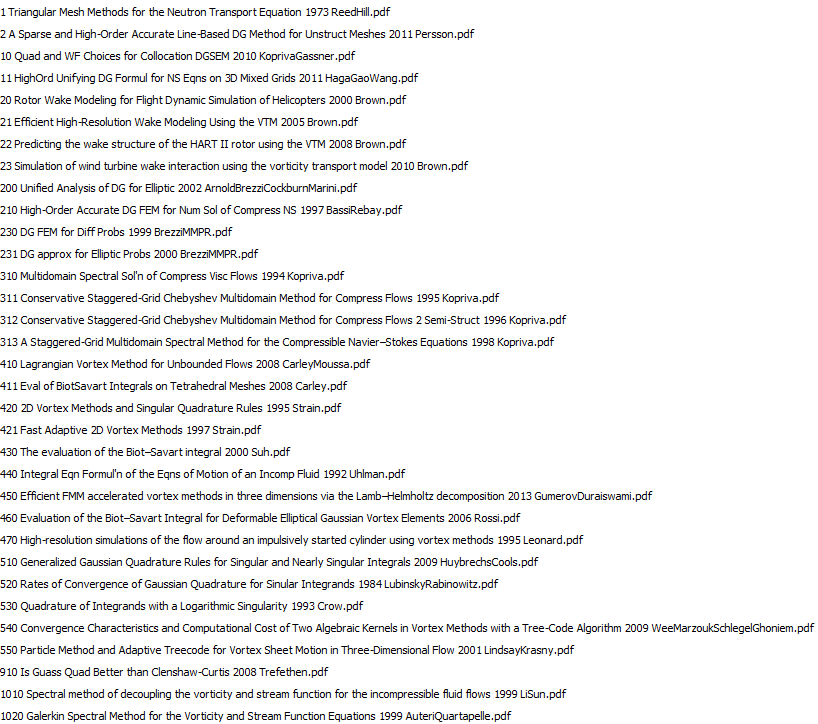
\includegraphics[width=1.4\textwidth]{LitStart.PNG}
%\caption{\label{fig:ring}Dirty preliminary lit cited.}
%\end{figure}
\end{document}